% ------------------------------------------------------------------
% Orynth v2 -- Bring-up sequence, bench to swarm.
% The risk-ordered operational counterpart to end_to_end_setup.pdf.
% Self-contained: all diagrams are TikZ, no external images required.
%
% Build:  pdflatex -interaction=nonstopmode bringup_sequence.tex
% (twice for cross-references and TOC)
% ------------------------------------------------------------------
\documentclass[11pt,a4paper]{article}

\usepackage[a4paper, margin=2cm, top=2.4cm, bottom=2.4cm]{geometry}
\usepackage{graphicx}
\usepackage{tikz}
\usetikzlibrary{shapes, shapes.geometric, shapes.symbols, shapes.multipart,
                arrows.meta, positioning, fit, backgrounds, calc,
                shadows.blur, decorations.pathreplacing, patterns,
                automata}
\usepackage{xcolor}
\usepackage{titlesec}
\usepackage[hidelinks]{hyperref}
\usepackage{enumitem}
\usepackage{caption}
\usepackage{tabularx}
\usepackage{array}
\usepackage{booktabs}
\usepackage{fancyhdr}
\usepackage{lmodern}
\usepackage{microtype}
\usepackage{titling}
\usepackage{tcolorbox}
\tcbuselibrary{skins, breakable}

% --- Brand colors (matches end_to_end_setup.tex) ---
\definecolor{fcblue}{HTML}{1f4e79}
\definecolor{rcorange}{HTML}{c75500}
\definecolor{jetsonteal}{HTML}{2e7d7d}
\definecolor{gcspurple}{HTML}{5a3370}
\definecolor{accentgreen}{HTML}{2e7d32}
\definecolor{bggrey}{HTML}{f4f4f4}
\definecolor{linegrey}{HTML}{555555}
\definecolor{lightaccent}{HTML}{e8eef5}
\definecolor{warnred}{HTML}{b3261e}
\definecolor{stagebg}{HTML}{f9f6ef}
\definecolor{stagerule}{HTML}{8a6d3b}

% --- TikZ styles ---
\tikzset{
  hwbox/.style={rectangle, draw=fcblue, fill=fcblue!8, very thick,
                rounded corners=3pt, minimum width=3.2cm, minimum height=1.2cm,
                align=center, font=\small},
  rcbox/.style={rectangle, draw=rcorange, fill=rcorange!10, very thick,
                rounded corners=3pt, minimum width=3.2cm, minimum height=1.2cm,
                align=center, font=\small},
  jetbox/.style={rectangle, draw=jetsonteal, fill=jetsonteal!10, very thick,
                 rounded corners=3pt, minimum width=3.2cm, minimum height=1.2cm,
                 align=center, font=\small},
  gcsbox/.style={rectangle, draw=gcspurple, fill=gcspurple!10, very thick,
                 rounded corners=3pt, minimum width=3.2cm, minimum height=1.2cm,
                 align=center, font=\small},
  fcbox/.style={rectangle, draw=fcblue, fill=fcblue!15, very thick,
                minimum width=3cm, minimum height=1.4cm,
                align=center, font=\small\bfseries},
  swcomp/.style={rectangle, draw=jetsonteal, fill=jetsonteal!8, thick,
                 minimum width=3.6cm, minimum height=1.1cm, align=center, font=\small},
  drone/.style={rectangle, draw=fcblue, fill=lightaccent, very thick,
                rounded corners=4pt, minimum width=2.1cm, minimum height=1.5cm,
                align=center, font=\scriptsize, drop shadow},
  ddsnode/.style={circle, draw=accentgreen, fill=accentgreen!10, thick,
                  minimum size=0.5cm, inner sep=0},
  link/.style={->, very thick, >={Stealth[length=3mm,width=2mm]}, draw=linegrey},
  biglink/.style={<->, very thick, >={Stealth[length=3mm,width=2mm]}, draw=linegrey},
  faintlink/.style={->, thick, >={Stealth[length=2.5mm,width=1.7mm]}, draw=linegrey!70, dashed},
  linklabel/.style={font=\scriptsize\itshape, fill=white, inner sep=2pt},
  % sequence diagram styles
  sdactor/.style={draw=fcblue, very thick, fill=fcblue!10, font=\small\bfseries,
                  minimum width=2.7cm, minimum height=0.7cm, rounded corners=2pt, align=center},
  sdactorlight/.style={draw=jetsonteal, very thick, fill=jetsonteal!10, font=\small\bfseries,
                       minimum width=2.7cm, minimum height=0.7cm, rounded corners=2pt, align=center},
  sdactorops/.style={draw=gcspurple, very thick, fill=gcspurple!10, font=\small\bfseries,
                     minimum width=2.7cm, minimum height=0.7cm, rounded corners=2pt, align=center},
  lifeline/.style={dashed, draw=linegrey!60, thick},
  sdmsg/.style={->, very thick, >={Stealth[length=2.8mm,width=1.8mm]}, draw=linegrey},
  sdret/.style={->, thick, dashed, >={Stealth[length=2.5mm,width=1.5mm]}, draw=linegrey!80},
  sdself/.style={->, thick, >={Stealth[length=2mm,width=1.4mm]}, draw=linegrey},
  sdlab/.style={font=\scriptsize\ttfamily, fill=white, inner sep=2pt},
  sdlabit/.style={font=\scriptsize\itshape, fill=white, inner sep=2pt},
  notebox/.style={draw=warnred!70, fill=warnred!8, rounded corners=2pt,
                  font=\scriptsize\itshape, inner sep=4pt, align=center},
  activation/.style={draw=fcblue, fill=lightaccent, very thick},
  % activity diagram styles
  actstart/.style={circle, draw=accentgreen, fill=accentgreen, minimum size=0.5cm, inner sep=0},
  actend/.style={circle, draw=accentgreen, fill=accentgreen, minimum size=0.5cm, inner sep=0,
                 path picture={\fill[white] (path picture bounding box.center) circle (0.13cm);
                               \fill[accentgreen] (path picture bounding box.center) circle (0.08cm);}},
  actstep/.style={rectangle, draw=fcblue, very thick, fill=fcblue!8, rounded corners=6pt,
                  minimum width=4.5cm, minimum height=0.9cm, align=center, font=\small},
  actcheck/.style={diamond, draw=warnred, very thick, fill=warnred!8, aspect=2.2,
                   inner sep=2pt, font=\scriptsize, align=center},
  actjoin/.style={rectangle, draw=fcblue, fill=fcblue, minimum width=4cm, minimum height=0.1cm},
  % stage badge
  stagebadge/.style={draw=stagerule, fill=stagebg, very thick, rounded corners=4pt,
                    minimum width=1.7cm, minimum height=0.9cm, font=\bfseries\large,
                    align=center, drop shadow},
}

% --- Photo placeholder ---
\newcommand{\photoplaceholder}[3]{%
  \begin{center}
  \begin{tikzpicture}
    \node[draw=gray!60, line width=1pt, fill=bggrey,
          minimum width=#1 cm, minimum height=#2 cm,
          inner sep=0, align=center] (ph) {};
    \draw[draw=gray!35, dashed] (ph.south west) -- (ph.north east);
    \draw[draw=gray!35, dashed] (ph.south east) -- (ph.north west);
    \node[anchor=north, font=\small\itshape\color{gray!75}]
      at ([yshift=-0.45cm]ph.north) {[ photo placeholder ]};
    \node[anchor=south, font=\scriptsize\color{gray!75}, align=center,
          text width={#1 cm - 1cm}] at ([yshift=0.45cm]ph.south) {#3};
  \end{tikzpicture}
  \end{center}
}

% --- Stage banner ---
\newcommand{\stagebanner}[3]{%
  \begin{tcolorbox}[colback=stagebg, colframe=stagerule, boxrule=1pt, arc=3pt,
                    left=0.6cm, right=0.6cm, top=0.4cm, bottom=0.4cm,
                    fontupper=\large]
  \textbf{Stage #1 \,---\, #2}\\[2pt]
  \small\textcolor{linegrey}{Goal: #3}
  \end{tcolorbox}%
}

\title{\bfseries Orynth v2 \\ \Large Bring-Up Sequence: Bench to Swarm}
\author{\large Risk-ordered procedure --- diagrams, sequences, gates}
\date{Revision: \today}

\titleformat{\section}{\Large\bfseries\color{fcblue}}{\thesection.}{0.6em}{}
\titlespacing*{\section}{0pt}{0.4em}{0.6em}
\titleformat{\subsection}{\large\bfseries\color{jetsonteal}}{\thesubsection.}{0.5em}{}

\pagestyle{fancy}
\fancyhf{}
\fancyfoot[C]{\small\thepage}
\fancyhead[L]{\small\itshape Orynth v2 --- Bring-up Sequence}
\fancyhead[R]{\small\itshape Bench $\rightarrow$ Swarm}
\renewcommand{\headrulewidth}{0.3pt}

\begin{document}

% =================================================================
% TITLE PAGE
% =================================================================
\thispagestyle{empty}
\begin{tikzpicture}[remember picture, overlay]
  \fill[fcblue] (current page.north west) rectangle ([yshift=-3.5cm]current page.north east);
  \node[anchor=north west, text=white, font=\Huge\bfseries]
    at ([xshift=2cm,yshift=-1.2cm]current page.north west) {Orynth v2};
  \node[anchor=north west, text=white, font=\Large]
    at ([xshift=2cm,yshift=-2.4cm]current page.north west)
    {Bring-Up Sequence: Bench to Swarm};
\end{tikzpicture}

\vspace{5.5cm}

\begin{center}
  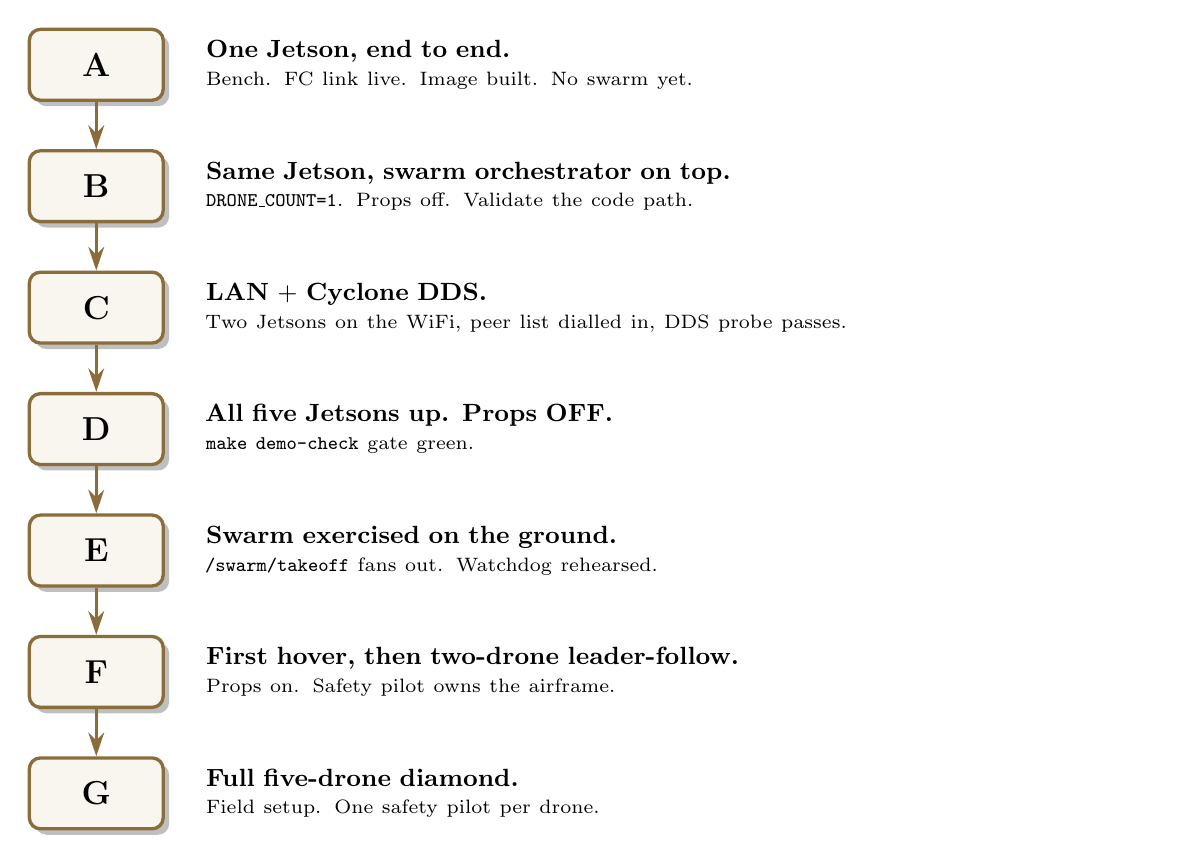
\begin{tikzpicture}[node distance=0.9cm, every node/.style={font=\small}]
    \node[stagebadge] (A) {A};
    \node[right=0.4cm of A, anchor=west, align=left, text width=12cm]
      {\textbf{One Jetson, end to end.}\\[-1pt]\scriptsize Bench. FC link live. Image built. No swarm yet.};
    \node[stagebadge, below=0.6cm of A] (B) {B};
    \node[right=0.4cm of B, anchor=west, align=left, text width=12cm]
      {\textbf{Same Jetson, swarm orchestrator on top.}\\[-1pt]\scriptsize \texttt{DRONE\_COUNT=1}. Props off. Validate the code path.};
    \node[stagebadge, below=0.6cm of B] (C) {C};
    \node[right=0.4cm of C, anchor=west, align=left, text width=12cm]
      {\textbf{LAN $+$ Cyclone DDS.}\\[-1pt]\scriptsize Two Jetsons on the WiFi, peer list dialled in, DDS probe passes.};
    \node[stagebadge, below=0.6cm of C] (D) {D};
    \node[right=0.4cm of D, anchor=west, align=left, text width=12cm]
      {\textbf{All five Jetsons up. Props OFF.}\\[-1pt]\scriptsize \texttt{make demo-check} gate green.};
    \node[stagebadge, below=0.6cm of D] (E) {E};
    \node[right=0.4cm of E, anchor=west, align=left, text width=12cm]
      {\textbf{Swarm exercised on the ground.}\\[-1pt]\scriptsize \texttt{/swarm/takeoff} fans out. Watchdog rehearsed.};
    \node[stagebadge, below=0.6cm of E] (F) {F};
    \node[right=0.4cm of F, anchor=west, align=left, text width=12cm]
      {\textbf{First hover, then two-drone leader-follow.}\\[-1pt]\scriptsize Props on. Safety pilot owns the airframe.};
    \node[stagebadge, below=0.6cm of F] (G) {G};
    \node[right=0.4cm of G, anchor=west, align=left, text width=12cm]
      {\textbf{Full five-drone diamond.}\\[-1pt]\scriptsize Field setup. One safety pilot per drone.};

    \draw[->, very thick, >={Stealth[length=3mm,width=2mm]}, draw=stagerule]
      (A.south) -- (B.north);
    \draw[->, very thick, >={Stealth[length=3mm,width=2mm]}, draw=stagerule]
      (B.south) -- (C.north);
    \draw[->, very thick, >={Stealth[length=3mm,width=2mm]}, draw=stagerule]
      (C.south) -- (D.north);
    \draw[->, very thick, >={Stealth[length=3mm,width=2mm]}, draw=stagerule]
      (D.south) -- (E.north);
    \draw[->, very thick, >={Stealth[length=3mm,width=2mm]}, draw=stagerule]
      (E.south) -- (F.north);
    \draw[->, very thick, >={Stealth[length=3mm,width=2mm]}, draw=stagerule]
      (F.south) -- (G.north);
  \end{tikzpicture}
\end{center}

\vfill
\noindent\textit{Companion to:\\
\texttt{docs/architecture/end\_to\_end/end\_to\_end\_setup.pdf} -- architecture.\\
\texttt{docs/runbooks/jetson\_swarm\_operations.md} -- per-command reference.\\[4pt]
This document is the {\bfseries operational, risk-ordered} view: what to do,
in what order, with what gate at each step.}

\vspace{0.5cm}
\hrule

\newpage

% =================================================================
% TOC
% =================================================================
\tableofcontents
\thispagestyle{fancy}
\newpage

% =================================================================
% PHILOSOPHY
% =================================================================
\section{The principle: earn each new variable}

The SITL stack proves software, not hardware. Moving to airframes adds five
new failure modes the simulator cannot reproduce: serial wiring, FC parameter
drift, the wireless LAN, multi-drone DDS discovery, and the airframe itself.
Each stage in this document is sized to add \emph{one} of those at a time,
with a gate at the end before the next stage starts.

\begin{center}
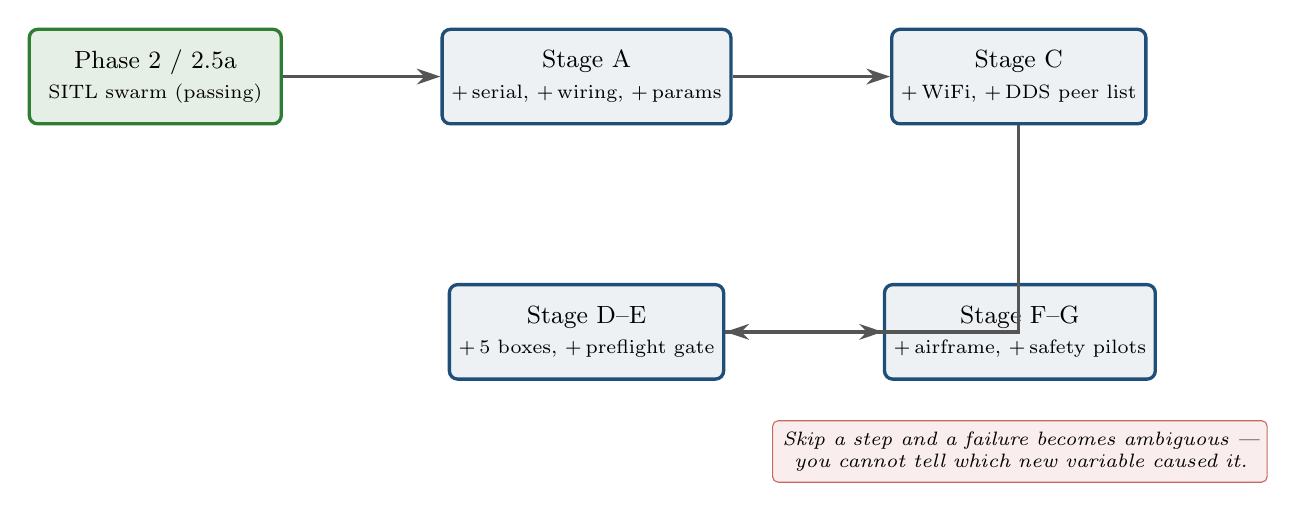
\begin{tikzpicture}[node distance=0.6cm and 1cm]
  \node[hwbox, fill=accentgreen!12, draw=accentgreen]
    (sitl) {Phase 2 / 2.5a\\\scriptsize SITL swarm (passing)};
  \node[hwbox, right=2cm of sitl] (stageA) {Stage A\\\scriptsize +\,serial, +\,wiring, +\,params};
  \node[hwbox, right=2cm of stageA] (stageC) {Stage C\\\scriptsize +\,WiFi, +\,DDS peer list};
  \node[hwbox, below=2cm of stageA] (stageD) {Stage D--E\\\scriptsize +\,5 boxes, +\,preflight gate};
  \node[hwbox, right=2cm of stageD] (stageF) {Stage F--G\\\scriptsize +\,airframe, +\,safety pilots};

  \draw[link] (sitl) -- (stageA);
  \draw[link] (stageA) -- (stageC);
  \draw[link] (stageC) |- (stageD);
  \draw[link] (stageD) -- (stageF);

  \node[notebox, below=0.5cm of stageF, text width=6cm]
    {Skip a step and a failure becomes ambiguous --- you cannot tell which new variable caused it.};
\end{tikzpicture}
\end{center}

\vspace{0.4cm}
\noindent\textbf{The two reference documents.} Throughout this guide:

\begin{itemize}[leftmargin=*, itemsep=2pt]
  \item \texttt{docs/architecture/end\_to\_end/end\_to\_end\_setup.pdf} ---
        the big picture: what runs where, why.
  \item \texttt{docs/runbooks/jetson\_swarm\_operations.md} --- the per-command
        reference with the troubleshooting table.
\end{itemize}

\noindent This document sequences \emph{when} to do each thing, and what
"pass" looks like before you move on.

\newpage

% =================================================================
% STAGE A
% =================================================================
\section{Stage A --- One Jetson, end to end}
\stagebanner{A}{Single Jetson, single FC, on the bench}{a single companion talks to a single ArduPilot FC over MAVROS, with the base image built and healthcheck green.}

\subsection{Deployment view}

\begin{center}
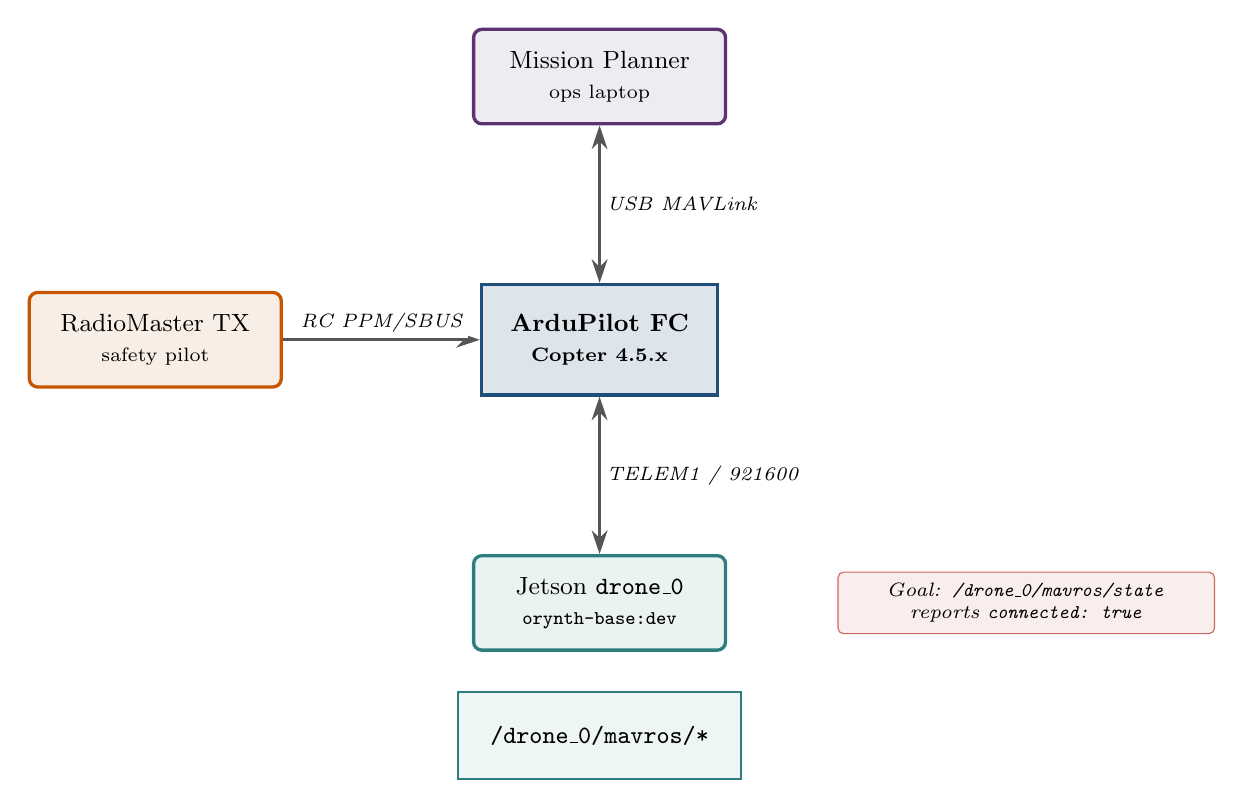
\begin{tikzpicture}[node distance=1.4cm]
  \node[gcsbox] (mp) {Mission Planner\\\scriptsize ops laptop};
  \node[fcbox, below=2cm of mp] (fc) {ArduPilot FC\\\scriptsize Copter 4.5.x};
  \node[rcbox, left=2.5cm of fc] (rc) {RadioMaster TX\\\scriptsize safety pilot};
  \node[jetbox, below=2cm of fc] (jet) {Jetson \texttt{drone\_0}\\\scriptsize \texttt{orynth-base:dev}};
  \node[swcomp, below=0.5cm of jet] (mavros) {\texttt{/drone\_0/mavros/*}};

  \draw[biglink] (mp.south) -- node[linklabel, right]{USB MAVLink} (fc.north);
  \draw[link] (rc.east) -- node[linklabel, above]{RC PPM/SBUS} (fc.west);
  \draw[biglink] (fc.south) -- node[linklabel, right]{TELEM1 / 921600} (jet.north);

  \node[notebox, right=1.4cm of jet, text width=4.5cm]
    {Goal: \texttt{/drone\_0/mavros/state} reports \texttt{connected: true}};
\end{tikzpicture}
\end{center}

\subsection{Bring-up flow}

\begin{center}
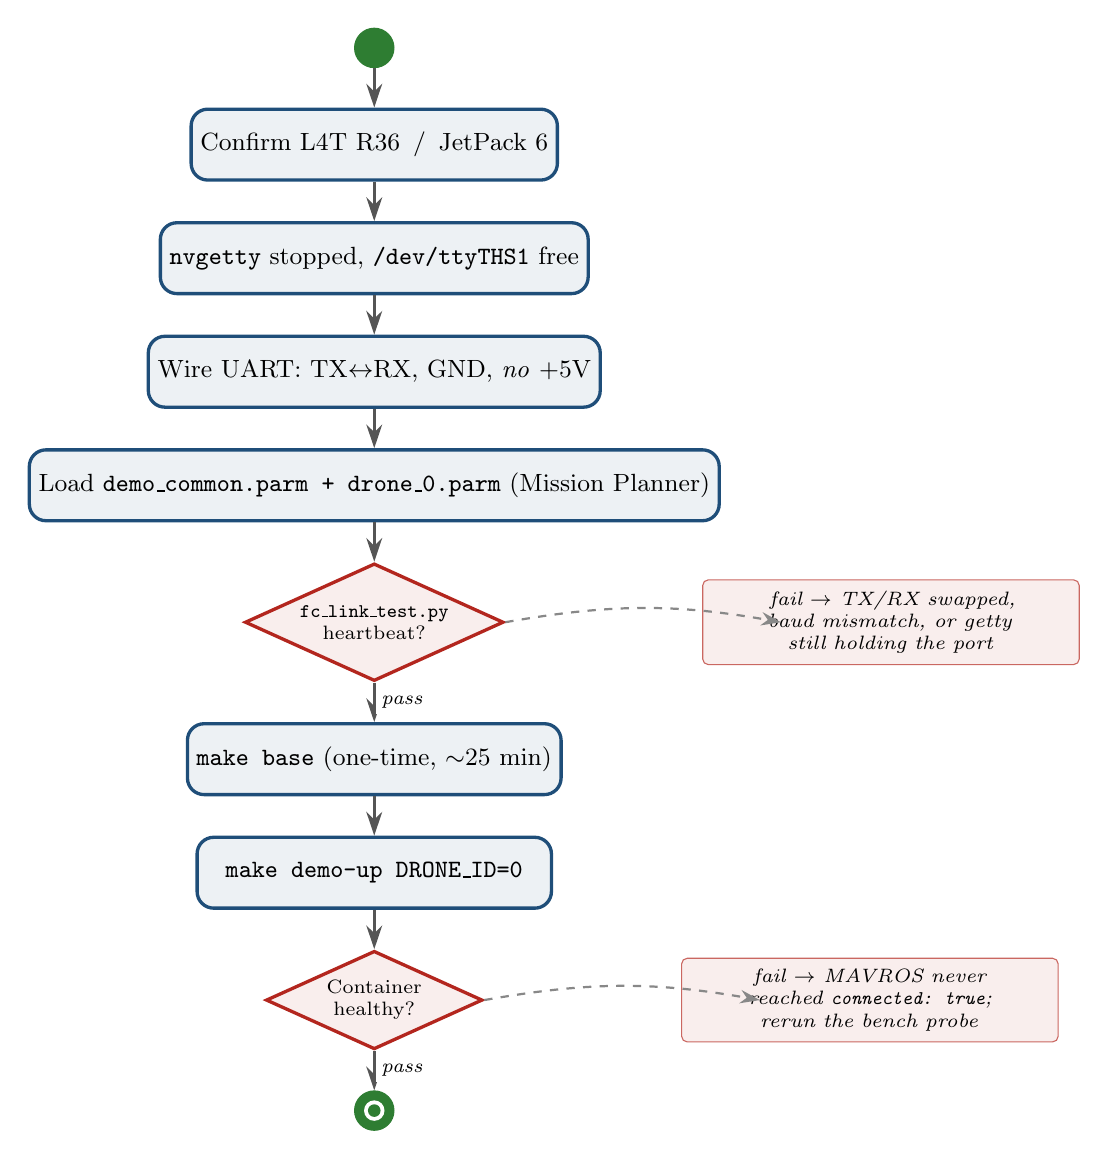
\begin{tikzpicture}[node distance=0.5cm]
  \node[actstart]              (s)                       {};
  \node[actstep, below=0.5cm of s]    (b)  {Confirm L4T R36 \,/\, JetPack 6};
  \node[actstep, below=of b]   (c)  {\texttt{nvgetty} stopped, \texttt{/dev/ttyTHS1} free};
  \node[actstep, below=of c]   (d)  {Wire UART: TX$\leftrightarrow$RX, GND, \emph{no} +5V};
  \node[actstep, below=of d]   (e)  {Load \texttt{demo\_common.parm + drone\_0.parm} (Mission Planner)};
  \node[actcheck, below=0.5cm of e]   (g1) {\texttt{fc\_link\_test.py}\\heartbeat?};
  \node[actstep, below=0.5cm of g1]   (f)  {\texttt{make base} (one-time, $\sim$25 min)};
  \node[actstep, below=of f]   (h)  {\texttt{make demo-up DRONE\_ID=0}};
  \node[actcheck, below=0.5cm of h]   (g2) {Container\\healthy?};
  \node[actend, below=0.5cm of g2]                   (end) {};

  \draw[link] (s) -- (b);
  \draw[link] (b) -- (c);
  \draw[link] (c) -- (d);
  \draw[link] (d) -- (e);
  \draw[link] (e) -- (g1);
  \draw[link] (g1) -- node[linklabel, right]{pass} (f);
  \draw[link] (f) -- (h);
  \draw[link] (h) -- (g2);
  \draw[link] (g2) -- node[linklabel, right]{pass} (end);

  \node[notebox, right=2.5cm of g1, text width=4.5cm]
    {fail $\rightarrow$ TX/RX swapped, baud mismatch, or getty still holding the port};
  \draw[faintlink] (g1.east) to[bend left=10] ($(g1.east) + (3.5,0)$);

  \node[notebox, right=2.5cm of g2, text width=4.5cm]
    {fail $\rightarrow$ MAVROS never reached \texttt{connected: true}; rerun the bench probe};
  \draw[faintlink] (g2.east) to[bend left=10] ($(g2.east) + (3.5,0)$);
\end{tikzpicture}
\end{center}

\subsection{What happens inside, on \texttt{make demo-up}}

\begin{center}
\resizebox{\textwidth}{!}{%
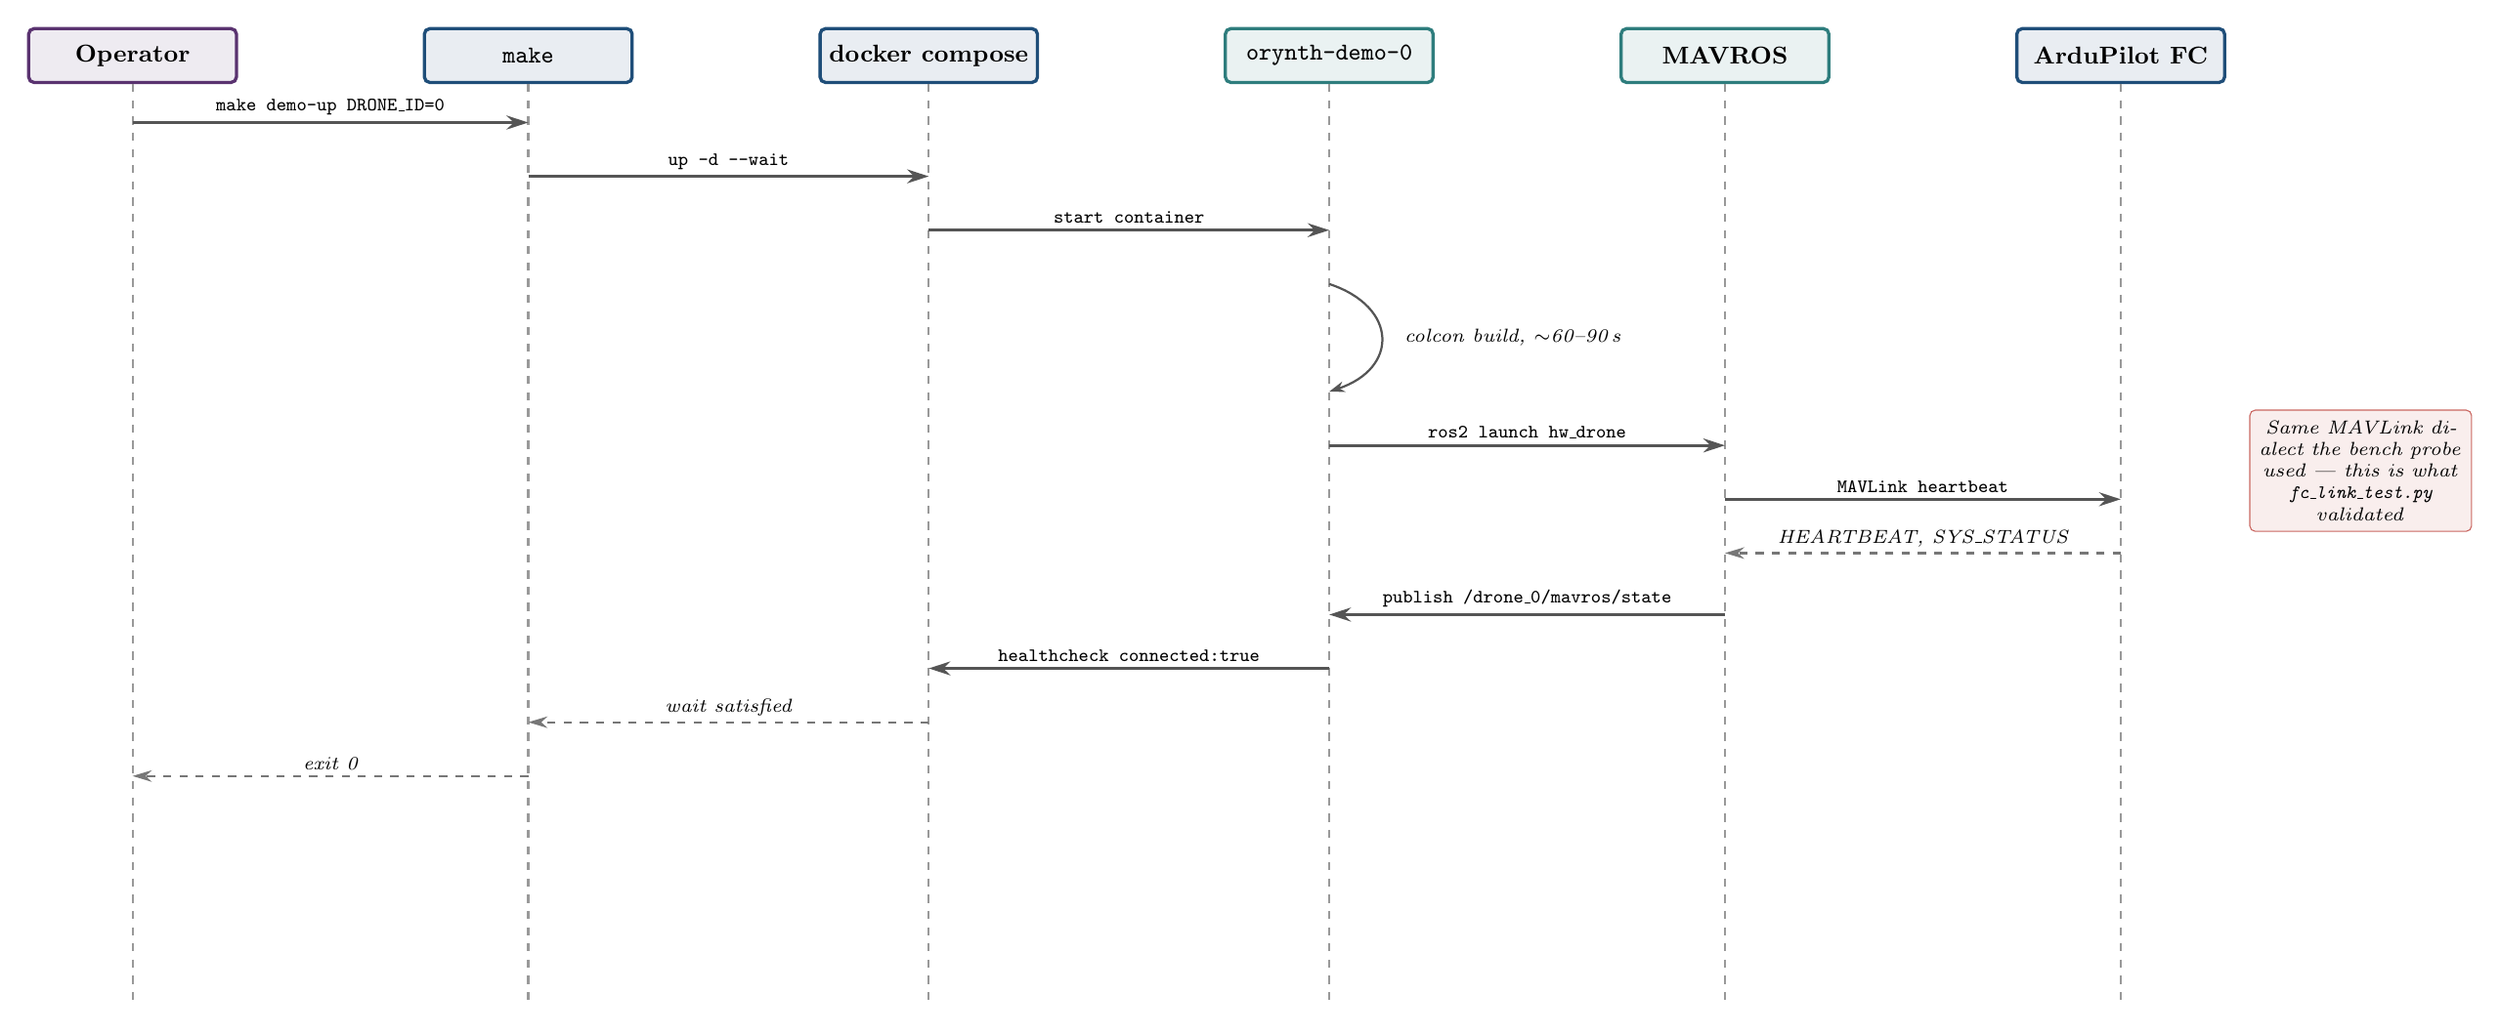
\begin{tikzpicture}[node distance=2.4cm]
  \node[sdactorops] (op) {Operator};
  \node[sdactor, right=of op]  (make) {\texttt{make}};
  \node[sdactor, right=of make] (dc)  {docker compose};
  \node[sdactorlight, right=of dc] (cont) {\texttt{orynth-demo-0}};
  \node[sdactorlight, right=of cont] (mr) {MAVROS};
  \node[sdactor, right=of mr] (fc) {ArduPilot FC};

  \foreach \n in {op, make, dc, cont, mr, fc} {
    \draw[lifeline] (\n.south) -- ++(0,-12);
  }

  \draw[sdmsg] ($(op.south) + (0,-0.5)$)   -- node[sdlab, above]{make demo-up DRONE\_ID=0} ($(make.south) + (0,-0.5)$);
  \draw[sdmsg] ($(make.south) + (0,-1.2)$) -- node[sdlab, above]{up -d --wait} ($(dc.south) + (0,-1.2)$);
  \draw[sdmsg] ($(dc.south) + (0,-1.9)$)   -- node[sdlab, above]{start container} ($(cont.south) + (0,-1.9)$);
  \draw[sdself, ->] ($(cont.south) + (0,-2.6)$) .. controls ($(cont.south) + (0.9,-2.9)$) and ($(cont.south) + (0.9,-3.7)$) .. ($(cont.south) + (0,-4.0)$);
  \node[sdlabit, anchor=west] at ($(cont.south) + (0.9,-3.3)$) {colcon build, $\sim$60--90\,s};
  \draw[sdmsg] ($(cont.south) + (0,-4.7)$) -- node[sdlab, above]{ros2 launch hw\_drone} ($(mr.south) + (0,-4.7)$);
  \draw[sdmsg] ($(mr.south) + (0,-5.4)$) -- node[sdlab, above]{MAVLink heartbeat} ($(fc.south) + (0,-5.4)$);
  \draw[sdret] ($(fc.south) + (0,-6.1)$) -- node[sdlabit, above]{HEARTBEAT, SYS\_STATUS} ($(mr.south) + (0,-6.1)$);
  \draw[sdmsg] ($(mr.south) + (0,-6.9)$) -- node[sdlab, above]{publish /drone\_0/mavros/state} ($(cont.south) + (0,-6.9)$);
  \draw[sdmsg] ($(cont.south) + (0,-7.6)$) -- node[sdlab, above]{healthcheck connected:true} ($(dc.south) + (0,-7.6)$);
  \draw[sdret] ($(dc.south) + (0,-8.3)$) -- node[sdlabit, above]{wait satisfied} ($(make.south) + (0,-8.3)$);
  \draw[sdret] ($(make.south) + (0,-9.0)$) -- node[sdlabit, above]{exit 0} ($(op.south) + (0,-9.0)$);

  \node[notebox, right=0.3cm of fc, text width=2.6cm, anchor=west,
        yshift=-5.4cm]
    {Same MAVLink dialect the bench probe used --- this is what \texttt{fc\_link\_test.py} validated};
\end{tikzpicture}%
}
\end{center}

\begin{tcolorbox}[colback=accentgreen!8, colframe=accentgreen, boxrule=0.8pt, arc=2pt]
\textbf{Gate to leave Stage A:} \texttt{ros2 topic echo --once /drone\_0/mavros/state}
inside \texttt{orynth-demo-0} prints \texttt{connected: true}.
\end{tcolorbox}

\newpage

% =================================================================
% STAGE B
% =================================================================
\section{Stage B --- Add the swarm orchestrator}
\stagebanner{B}{Same Jetson, \texttt{swarm\_server} on top, props off}{the orchestrator code path runs end-to-end on real hardware before the network is involved.}

\noindent The single-drone case is also a \emph{degenerate swarm}: launch with
\texttt{DRONE\_COUNT=1} and \texttt{swarm\_server} orchestrates exactly one
airframe. This validates the whole code path without involving WiFi.

\subsection{Component view --- what runs on one Jetson}

\begin{center}
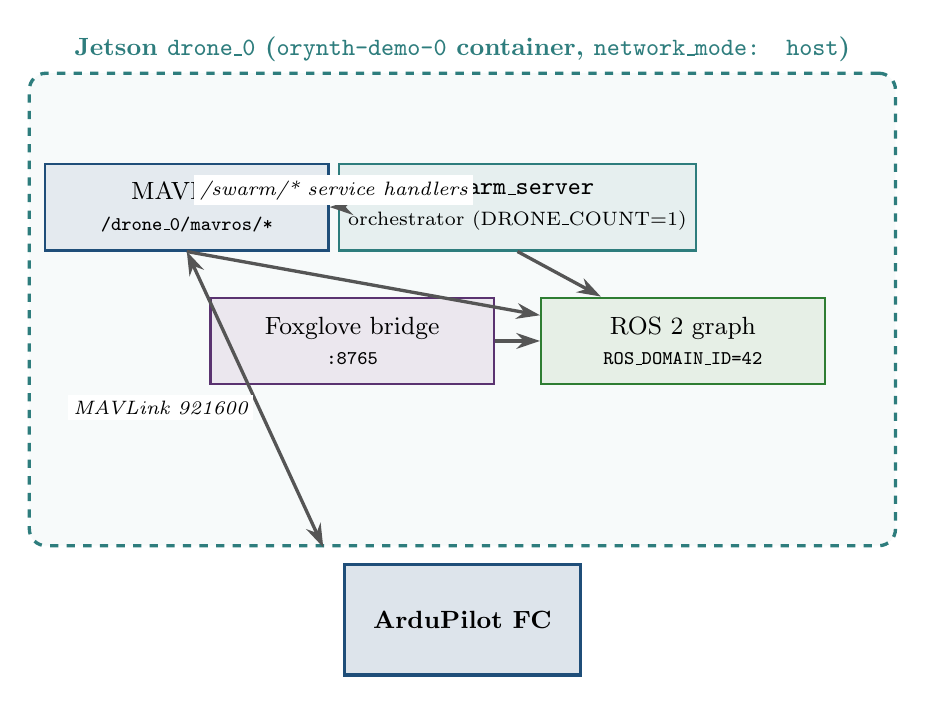
\begin{tikzpicture}[node distance=0.6cm]
  \node[draw=jetsonteal, very thick, dashed, fill=jetsonteal!4, rounded corners=6pt,
        minimum width=11cm, minimum height=6cm, label={[font=\small\bfseries\color{jetsonteal}]above:Jetson \texttt{drone\_0} (\texttt{orynth-demo-0} container, \texttt{network\_mode: host})}] (j) {};

  \node[swcomp, fill=fcblue!12, draw=fcblue] (mr) at ($(j.center) + (-3.5,1.3)$) {MAVROS\\\scriptsize \texttt{/drone\_0/mavros/*}};
  \node[swcomp, fill=jetsonteal!12] (ss) at ($(j.center) + (0.7,1.3)$) {\texttt{swarm\_server}\\\scriptsize orchestrator (DRONE\_COUNT=1)};
  \node[swcomp, fill=gcspurple!12, draw=gcspurple] (fb) at ($(j.center) + (-1.4,-0.4)$) {Foxglove bridge\\\scriptsize \texttt{:8765}};
  \node[swcomp, fill=accentgreen!12, draw=accentgreen] (ros) at ($(j.center) + (2.8,-0.4)$) {ROS 2 graph\\\scriptsize \texttt{ROS\_DOMAIN\_ID=42}};
  \node[fcbox, below=0.2cm of j.south, anchor=north] (fc) {ArduPilot FC};

  \draw[biglink] (mr.south) -- node[linklabel, left, yshift=-0.1cm]{MAVLink 921600} ($(j.south)!0.32!(j.south west)$);
  \draw[link] (ss) -- node[linklabel, above]{/swarm/* service handlers} (mr);
  \draw[link] (ss.south) -- (ros);
  \draw[link] (mr.south) -- (ros);
  \draw[link] (fb.east) -- (ros);
\end{tikzpicture}
\end{center}

\subsection{One service call, end to end}

\begin{center}
\resizebox{\textwidth}{!}{%
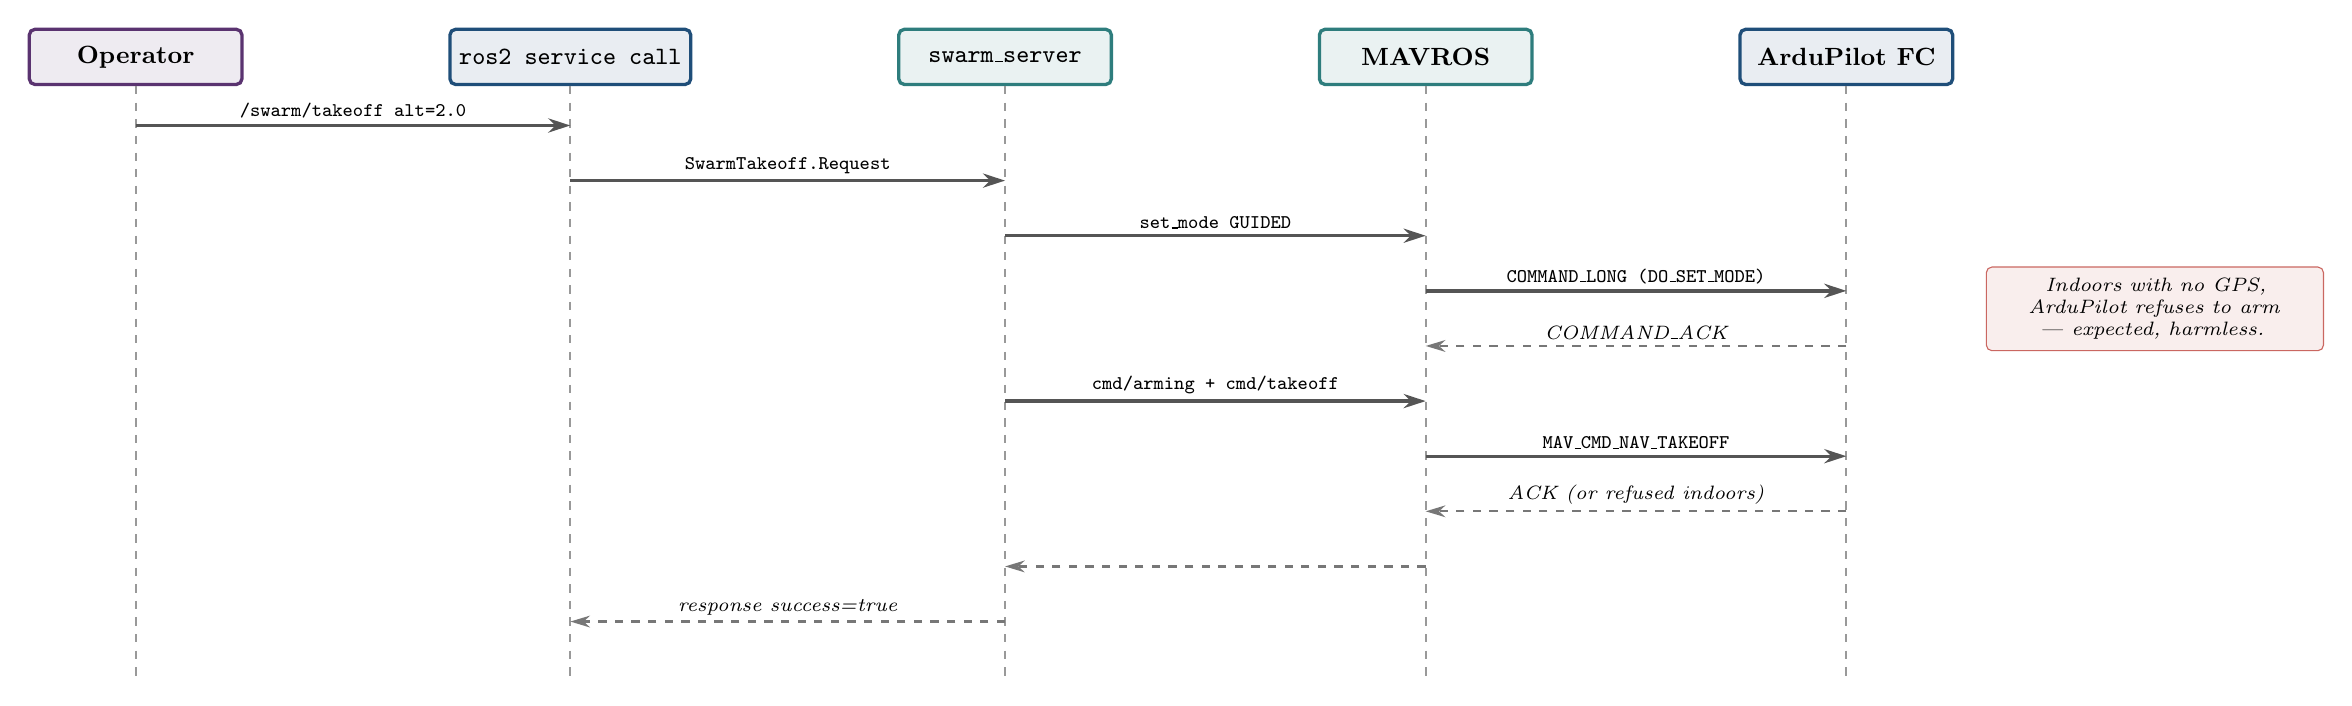
\begin{tikzpicture}[node distance=2.6cm]
  \node[sdactorops] (op) {Operator};
  \node[sdactor, right=of op] (cli) {\texttt{ros2 service call}};
  \node[sdactorlight, right=of cli] (ss) {\texttt{swarm\_server}};
  \node[sdactorlight, right=of ss] (mr) {MAVROS};
  \node[sdactor, right=of mr] (fc) {ArduPilot FC};

  \foreach \n in {op, cli, ss, mr, fc} {
    \draw[lifeline] (\n.south) -- ++(0,-7.5);
  }

  \draw[sdmsg] ($(op.south) + (0,-0.5)$) -- node[sdlab, above]{/swarm/takeoff alt=2.0} ($(cli.south) + (0,-0.5)$);
  \draw[sdmsg] ($(cli.south) + (0,-1.2)$) -- node[sdlab, above]{SwarmTakeoff.Request} ($(ss.south) + (0,-1.2)$);
  \draw[sdmsg] ($(ss.south) + (0,-1.9)$) -- node[sdlab, above]{set\_mode GUIDED} ($(mr.south) + (0,-1.9)$);
  \draw[sdmsg] ($(mr.south) + (0,-2.6)$) -- node[sdlab, above]{COMMAND\_LONG (DO\_SET\_MODE)} ($(fc.south) + (0,-2.6)$);
  \draw[sdret] ($(fc.south) + (0,-3.3)$) -- node[sdlabit, above]{COMMAND\_ACK} ($(mr.south) + (0,-3.3)$);
  \draw[sdmsg] ($(ss.south) + (0,-4.0)$) -- node[sdlab, above]{cmd/arming + cmd/takeoff} ($(mr.south) + (0,-4.0)$);
  \draw[sdmsg] ($(mr.south) + (0,-4.7)$) -- node[sdlab, above]{MAV\_CMD\_NAV\_TAKEOFF} ($(fc.south) + (0,-4.7)$);
  \draw[sdret] ($(fc.south) + (0,-5.4)$) -- node[sdlabit, above]{ACK (or refused indoors)} ($(mr.south) + (0,-5.4)$);
  \draw[sdret] ($(mr.south) + (0,-6.1)$) -- ($(ss.south) + (0,-6.1)$);
  \draw[sdret] ($(ss.south) + (0,-6.8)$) -- node[sdlabit, above]{response success=true} ($(cli.south) + (0,-6.8)$);

  \node[notebox, anchor=west, text width=4cm] at ($(fc.east) + (0.4,-3.2)$)
    {Indoors with no GPS, ArduPilot refuses to arm --- expected, harmless.};
\end{tikzpicture}%
}
\end{center}

\begin{tcolorbox}[colback=accentgreen!8, colframe=accentgreen, boxrule=0.8pt, arc=2pt]
\textbf{Gate to leave Stage B:} the FC switches to GUIDED, \texttt{/swarm/status}
walks through the takeoff phases, and \texttt{/swarm/land} returns it to STABILIZE.
Props off; arming indoors will fail and that is fine.
\end{tcolorbox}

\newpage

% =================================================================
% STAGE C
% =================================================================
\section{Stage C --- The LAN and Cyclone DDS}
\stagebanner{C}{Two Jetsons on WiFi, talking}{prove DDS discovery and per-drone Cyclone DDS config work before scaling to five.}

\noindent This is the stage that SITL cannot teach. Three facts shape it:
\begin{itemize}[leftmargin=*, itemsep=1pt]
  \item \texttt{network\_mode: host} is mandatory --- the Docker bridge cannot bridge DDS onto the physical WiFi.
  \item Most WiFi APs silently drop multicast. SPDP is multicast by default, so it does not arrive.
  \item The repo's answer is an \emph{explicit peer list} in \texttt{config/networks/cyclonedds\_drone\_template.xml}.
\end{itemize}

\subsection{Network topology --- the LAN you build}

\begin{center}
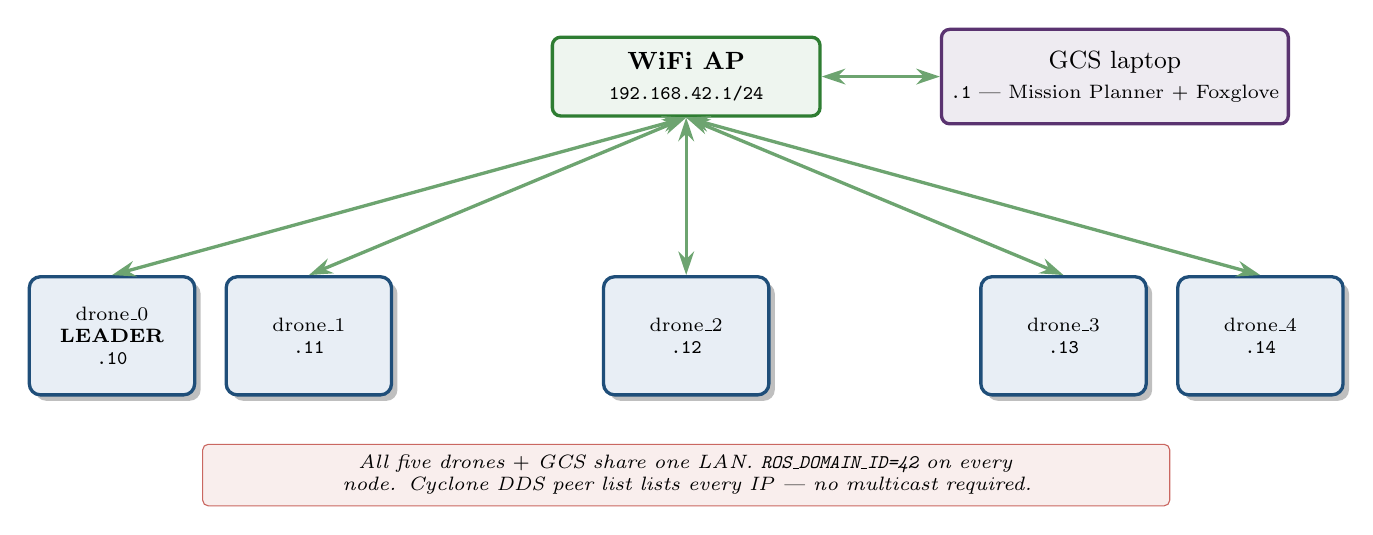
\begin{tikzpicture}[node distance=1.2cm]
  \node[rectangle, draw=accentgreen, very thick, fill=accentgreen!8,
        minimum width=3.4cm, minimum height=1.0cm, rounded corners=3pt,
        font=\small\bfseries, align=center] (ap)
    {WiFi AP\\\scriptsize \texttt{192.168.42.1/24}};

  \node[drone, below left=2cm and 4.5cm of ap] (d0) {drone\_0\\\textbf{LEADER}\\\scriptsize \texttt{.10}};
  \node[drone, below left=2cm and 2.0cm of ap] (d1) {drone\_1\\\scriptsize \texttt{.11}};
  \node[drone, below=2cm of ap] (d2) {drone\_2\\\scriptsize \texttt{.12}};
  \node[drone, below right=2cm and 2.0cm of ap] (d3) {drone\_3\\\scriptsize \texttt{.13}};
  \node[drone, below right=2cm and 4.5cm of ap] (d4) {drone\_4\\\scriptsize \texttt{.14}};
  \node[gcsbox, right=1.5cm of ap] (gcs) {GCS laptop\\\scriptsize \texttt{.1} --- Mission Planner + Foxglove};

  \foreach \n in {d0, d1, d2, d3, d4} {
    \draw[biglink, draw=accentgreen!70] (\n.north) -- (ap.south);
  }
  \draw[biglink, draw=accentgreen!70] (gcs.west) -- (ap.east);

  \node[notebox, below=0.6cm of d2, text width=12cm]
    {All five drones $+$ GCS share one LAN. \texttt{ROS\_DOMAIN\_ID=42} on every node.
     Cyclone DDS peer list lists every IP --- no multicast required.};
\end{tikzpicture}
\end{center}

\subsection{Why the peer list --- multicast SPDP vs unicast SPDP}

\begin{center}
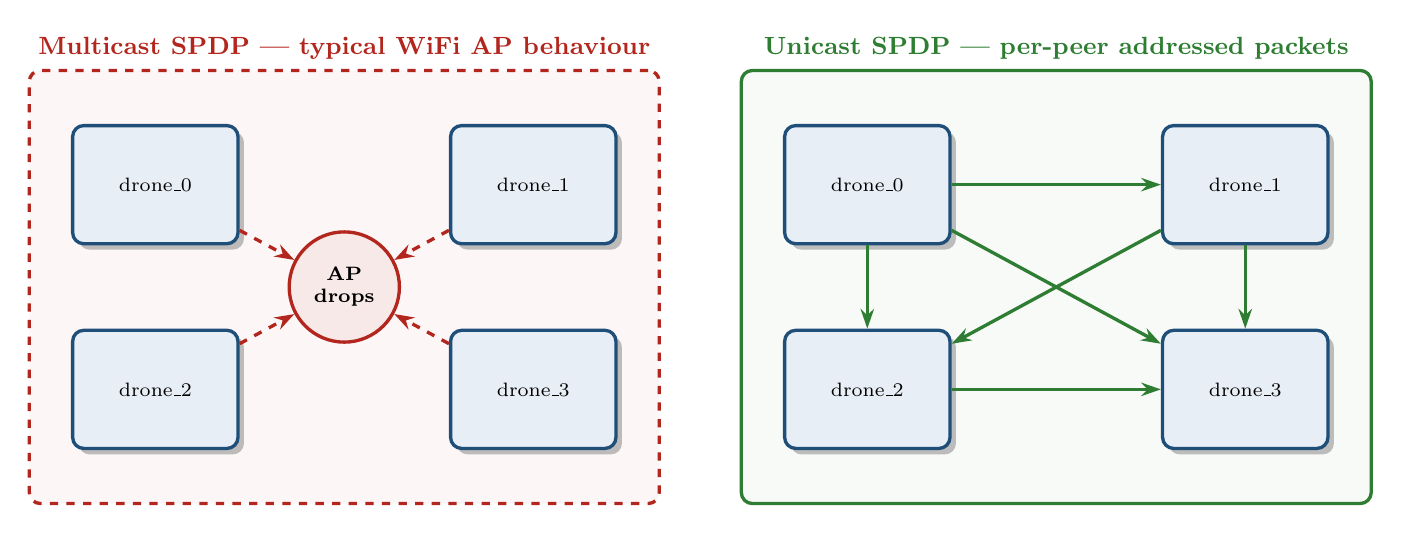
\begin{tikzpicture}[node distance=1.2cm]
  % --- LEFT: multicast (broken) ---
  \node[rectangle, draw=warnred, very thick, dashed, fill=warnred!4, rounded corners=4pt,
        minimum width=8cm, minimum height=5.5cm,
        label={[font=\small\bfseries\color{warnred}]above:Multicast SPDP --- typical WiFi AP behaviour}] (left) {};
  \node[drone] (l0) at ($(left.center) + (-2.4, 1.3)$) {drone\_0};
  \node[drone] (l1) at ($(left.center) + (2.4, 1.3)$)  {drone\_1};
  \node[drone] (l2) at ($(left.center) + (-2.4, -1.3)$) {drone\_2};
  \node[drone] (l3) at ($(left.center) + (2.4, -1.3)$)  {drone\_3};
  \node[circle, draw=warnred, very thick, fill=warnred!10, minimum size=1.4cm,
        font=\scriptsize\bfseries, align=center, inner sep=1pt] (X) at (left.center)
        {AP\\drops};

  \foreach \n in {l0, l1, l2, l3} {
    \draw[->, very thick, draw=warnred, dashed,
          >={Stealth[length=2.5mm,width=1.7mm]}] (\n) -- (X);
  }

  % --- RIGHT: unicast (working) ---
  \node[rectangle, draw=accentgreen, very thick, fill=accentgreen!4, rounded corners=4pt,
        minimum width=8cm, minimum height=5.5cm, right=1cm of left,
        label={[font=\small\bfseries\color{accentgreen}]above:Unicast SPDP --- per-peer addressed packets}] (right) {};
  \node[drone] (r0) at ($(right.center) + (-2.4, 1.3)$) {drone\_0};
  \node[drone] (r1) at ($(right.center) + (2.4, 1.3)$)  {drone\_1};
  \node[drone] (r2) at ($(right.center) + (-2.4, -1.3)$) {drone\_2};
  \node[drone] (r3) at ($(right.center) + (2.4, -1.3)$)  {drone\_3};

  \draw[->, very thick, draw=accentgreen, >={Stealth[length=2.5mm,width=1.7mm]}]
    (r0) -- (r1);
  \draw[->, very thick, draw=accentgreen, >={Stealth[length=2.5mm,width=1.7mm]}]
    (r0) -- (r2);
  \draw[->, very thick, draw=accentgreen, >={Stealth[length=2.5mm,width=1.7mm]}]
    (r0) -- (r3);
  \draw[->, very thick, draw=accentgreen, >={Stealth[length=2.5mm,width=1.7mm]}]
    (r1) -- (r2);
  \draw[->, very thick, draw=accentgreen, >={Stealth[length=2.5mm,width=1.7mm]}]
    (r1) -- (r3);
  \draw[->, very thick, draw=accentgreen, >={Stealth[length=2.5mm,width=1.7mm]}]
    (r2) -- (r3);
\end{tikzpicture}
\end{center}

\subsection{The peer-list config (per Jetson)}

\begin{center}
\begin{tcolorbox}[colback=bggrey, colframe=fcblue!60, boxrule=0.6pt, arc=2pt,
                  width=15cm, fontupper=\scriptsize\ttfamily]
\textcolor{linegrey}{\itshape config/networks/cyclonedds\_drone\_0.xml}\\[2pt]
<CycloneDDS>\\
\quad<Domain id="any">\\
\quad\quad<General>\\
\quad\quad\quad<NetworkInterfaceAddress>wlan0</NetworkInterfaceAddress>\\
\quad\quad\quad<AllowMulticast>spdp</AllowMulticast>  \textcolor{linegrey}{\itshape <!-- fall back to "false" if AP hostile -->}\\
\quad\quad</General>\\
\quad\quad<Discovery>\\
\quad\quad\quad<Peers>\\
\quad\quad\quad\quad<Peer address="192.168.42.10"/>  \textcolor{linegrey}{\itshape <!-- drone\_0 (leader) -->}\\
\quad\quad\quad\quad<Peer address="192.168.42.11"/>  \textcolor{linegrey}{\itshape <!-- drone\_1 -->}\\
\quad\quad\quad\quad<Peer address="192.168.42.12"/>  \textcolor{linegrey}{\itshape <!-- drone\_2 -->}\\
\quad\quad\quad\quad<Peer address="192.168.42.13"/>  \textcolor{linegrey}{\itshape <!-- drone\_3 -->}\\
\quad\quad\quad\quad<Peer address="192.168.42.14"/>  \textcolor{linegrey}{\itshape <!-- drone\_4 -->}\\
\quad\quad\quad\quad<Peer address="192.168.42.1"/>   \textcolor{linegrey}{\itshape <!-- gcs laptop -->}\\
\quad\quad\quad</Peers>\\
\quad\quad</Discovery>\\
\quad</Domain>\\
</CycloneDDS>
\end{tcolorbox}
\end{center}

\subsection{Two-node DDS probe before scaling}

Bring up two Jetsons (any pair), \emph{outside} the demo stack to isolate DDS
from MAVROS. On each:

\begin{center}
\begin{tcolorbox}[colback=bggrey, colframe=fcblue!60, boxrule=0.6pt, arc=2pt,
                  width=15cm, fontupper=\footnotesize\ttfamily]
\textcolor{linegrey}{\itshape \# Jetson \#0:}\\
CYCLONEDDS\_URI=file://\$PWD/config/networks/cyclonedds\_drone\_0.xml \textbackslash\\
ROS\_DOMAIN\_ID=42 RMW\_IMPLEMENTATION=rmw\_cyclonedds\_cpp \textbackslash\\
ros2 topic pub -r1 /\_\_dds\_probe std\_msgs/msg/String '{data: hello}'\\[6pt]
\textcolor{linegrey}{\itshape \# Jetson \#1:}\\
CYCLONEDDS\_URI=file://\$PWD/config/networks/cyclonedds\_drone\_1.xml \textbackslash\\
ROS\_DOMAIN\_ID=42 RMW\_IMPLEMENTATION=rmw\_cyclonedds\_cpp \textbackslash\\
ros2 topic echo /\_\_dds\_probe
\end{tcolorbox}
\end{center}

\begin{tcolorbox}[colback=accentgreen!8, colframe=accentgreen, boxrule=0.8pt, arc=2pt]
\textbf{Gate to leave Stage C:} \texttt{hello} flows from \#0 to \#1 (and back the
other way). If this does not work, no demo bringup will. Most common cause:
client isolation on the AP, or \texttt{NetworkInterfaceAddress} naming the wrong iface.
\end{tcolorbox}

\newpage

% =================================================================
% STAGE D
% =================================================================
\section{Stage D --- All five Jetsons up, props OFF}
\stagebanner{D}{Five companions discovered, preflight gate green}{the swarm orchestrator on the leader sees and queries all four followers.}

\subsection{Deployment view --- all five}

\begin{center}
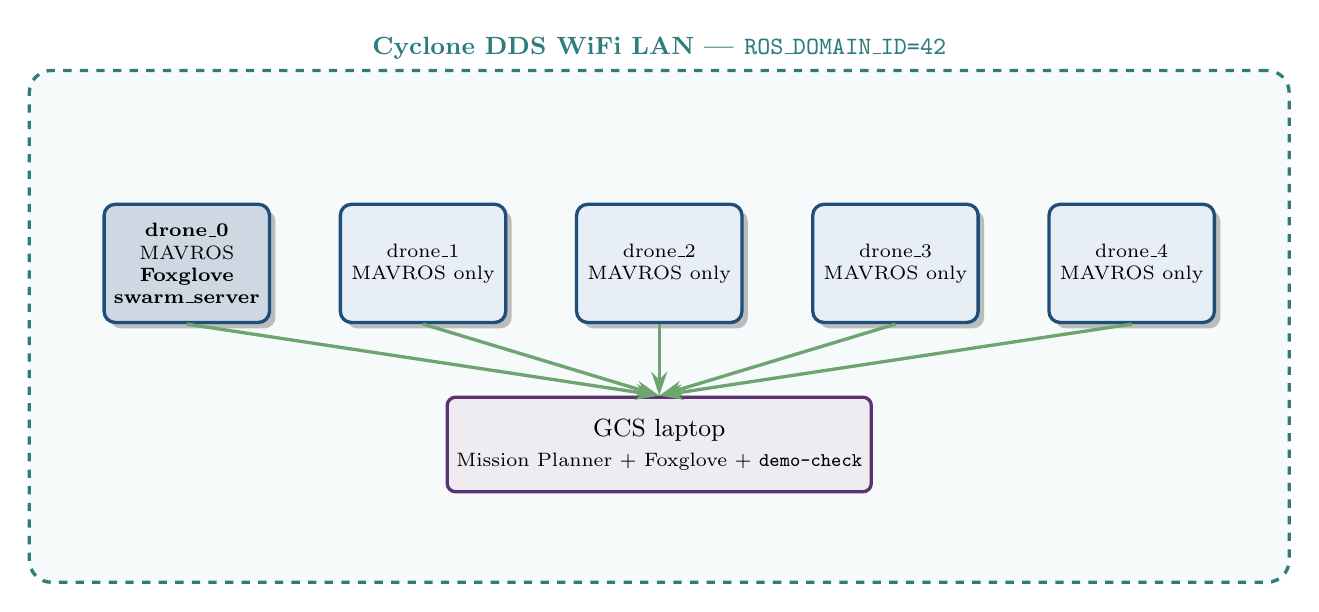
\begin{tikzpicture}[node distance=1.3cm]
  \node[draw=jetsonteal, very thick, dashed, fill=jetsonteal!4, rounded corners=8pt,
        minimum width=16cm, minimum height=6.5cm,
        label={[font=\small\bfseries\color{jetsonteal}]above:Cyclone DDS WiFi LAN --- \texttt{ROS\_DOMAIN\_ID=42}}] (lan) {};

  \node[drone, fill=fcblue!22] (d0) at ($(lan.center) + (-6, 0.8)$)
    {\textbf{drone\_0}\\\scriptsize MAVROS\\\scriptsize \textbf{Foxglove}\\\scriptsize \textbf{swarm\_server}};
  \node[drone] (d1) at ($(lan.center) + (-3, 0.8)$) {drone\_1\\\scriptsize MAVROS only};
  \node[drone] (d2) at ($(lan.center) + (0, 0.8)$)  {drone\_2\\\scriptsize MAVROS only};
  \node[drone] (d3) at ($(lan.center) + (3, 0.8)$)  {drone\_3\\\scriptsize MAVROS only};
  \node[drone] (d4) at ($(lan.center) + (6, 0.8)$)  {drone\_4\\\scriptsize MAVROS only};
  \node[gcsbox] (gcs) at ($(lan.center) + (0, -1.5)$)
    {GCS laptop\\\scriptsize Mission Planner $+$ Foxglove $+$ \texttt{demo-check}};

  \foreach \n in {d0, d1, d2, d3, d4} {
    \draw[link, draw=accentgreen!70] (\n.south) -- (gcs.north);
  }
\end{tikzpicture}
\end{center}

\subsection{The preflight gate --- what \texttt{make demo-check} runs}

\begin{center}
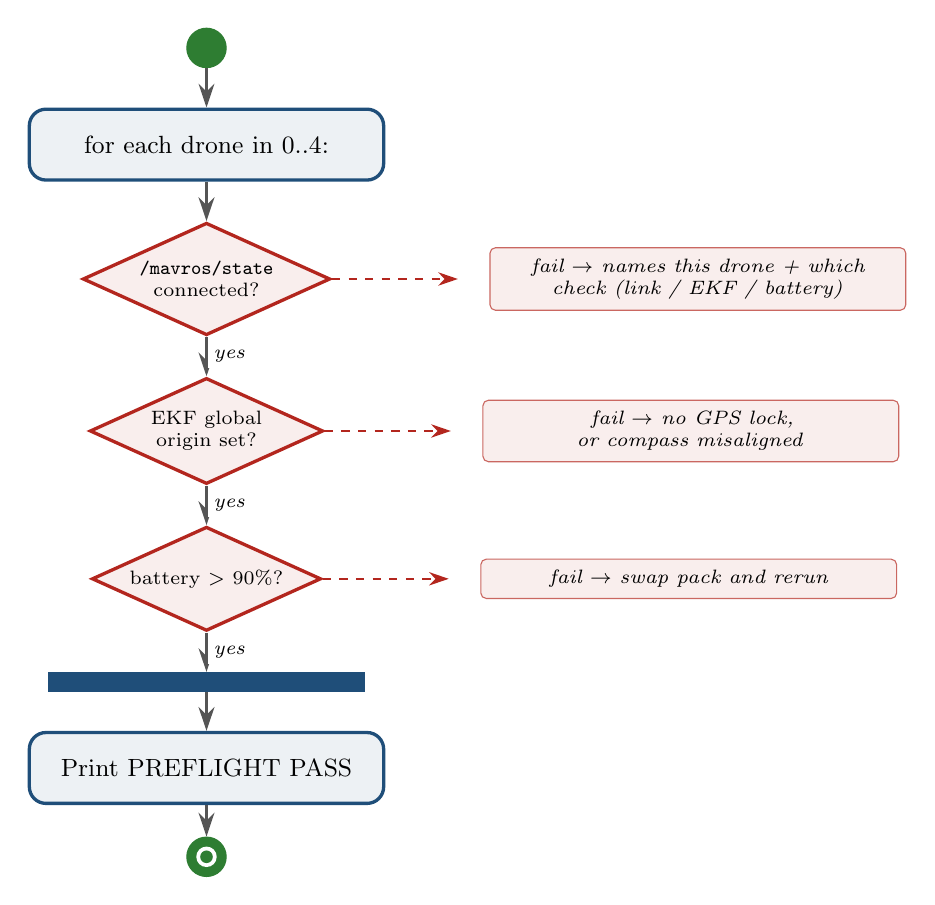
\begin{tikzpicture}[node distance=0.5cm]
  \node[actstart] (s) {};
  \node[actstep, below=of s] (loop) {for each drone in 0..4:};

  \node[actcheck, below=0.5cm of loop] (g1) {\texttt{/mavros/state}\\connected?};
  \node[actcheck, below=0.5cm of g1] (g2) {EKF global\\origin set?};
  \node[actcheck, below=0.5cm of g2] (g3) {battery $>$ 90\%?};
  \node[actjoin, below=0.5cm of g3] (j) {};
  \node[actstep, below=0.5cm of j] (pass) {Print PREFLIGHT PASS};
  \node[actend, below=0.4cm of pass] (e) {};

  \draw[link] (s) -- (loop);
  \draw[link] (loop) -- (g1);
  \draw[link] (g1) -- node[linklabel, right]{yes} (g2);
  \draw[link] (g2) -- node[linklabel, right]{yes} (g3);
  \draw[link] (g3) -- node[linklabel, right]{yes} (j);
  \draw[link] (j) -- (pass);
  \draw[link] (pass) -- (e);

  \node[notebox, right=2cm of g1, text width=5cm]
    {fail $\rightarrow$ names this drone + which check (link / EKF / battery)};
  \node[notebox, right=2cm of g2, text width=5cm]
    {fail $\rightarrow$ no GPS lock, or compass misaligned};
  \node[notebox, right=2cm of g3, text width=5cm]
    {fail $\rightarrow$ swap pack and rerun};
  \draw[faintlink, draw=warnred] (g1.east) -- ++(1.6,0);
  \draw[faintlink, draw=warnred] (g2.east) -- ++(1.6,0);
  \draw[faintlink, draw=warnred] (g3.east) -- ++(1.6,0);
\end{tikzpicture}
\end{center}

\begin{tcolorbox}[colback=accentgreen!8, colframe=accentgreen, boxrule=0.8pt, arc=2pt]
\textbf{Gate to leave Stage D:} \texttt{make demo-check} prints
\texttt{PREFLIGHT PASS}, all five \texttt{/drone\_<N>/mavros/state} reported
\texttt{connected: true}, and Foxglove (\texttt{ws://192.168.42.10:8765})
shows five poses.
\end{tcolorbox}

\newpage

% =================================================================
% STAGE E
% =================================================================
\section{Stage E --- Exercise the swarm without flying}
\stagebanner{E}{Props OFF on all five, \texttt{/swarm/takeoff} fans out}{the orchestrator reaches every follower over DDS, and the watchdog is rehearsed.}

\subsection{\texttt{/swarm/takeoff} fan-out --- one call, five FCs}

\begin{center}
\resizebox{\textwidth}{!}{%
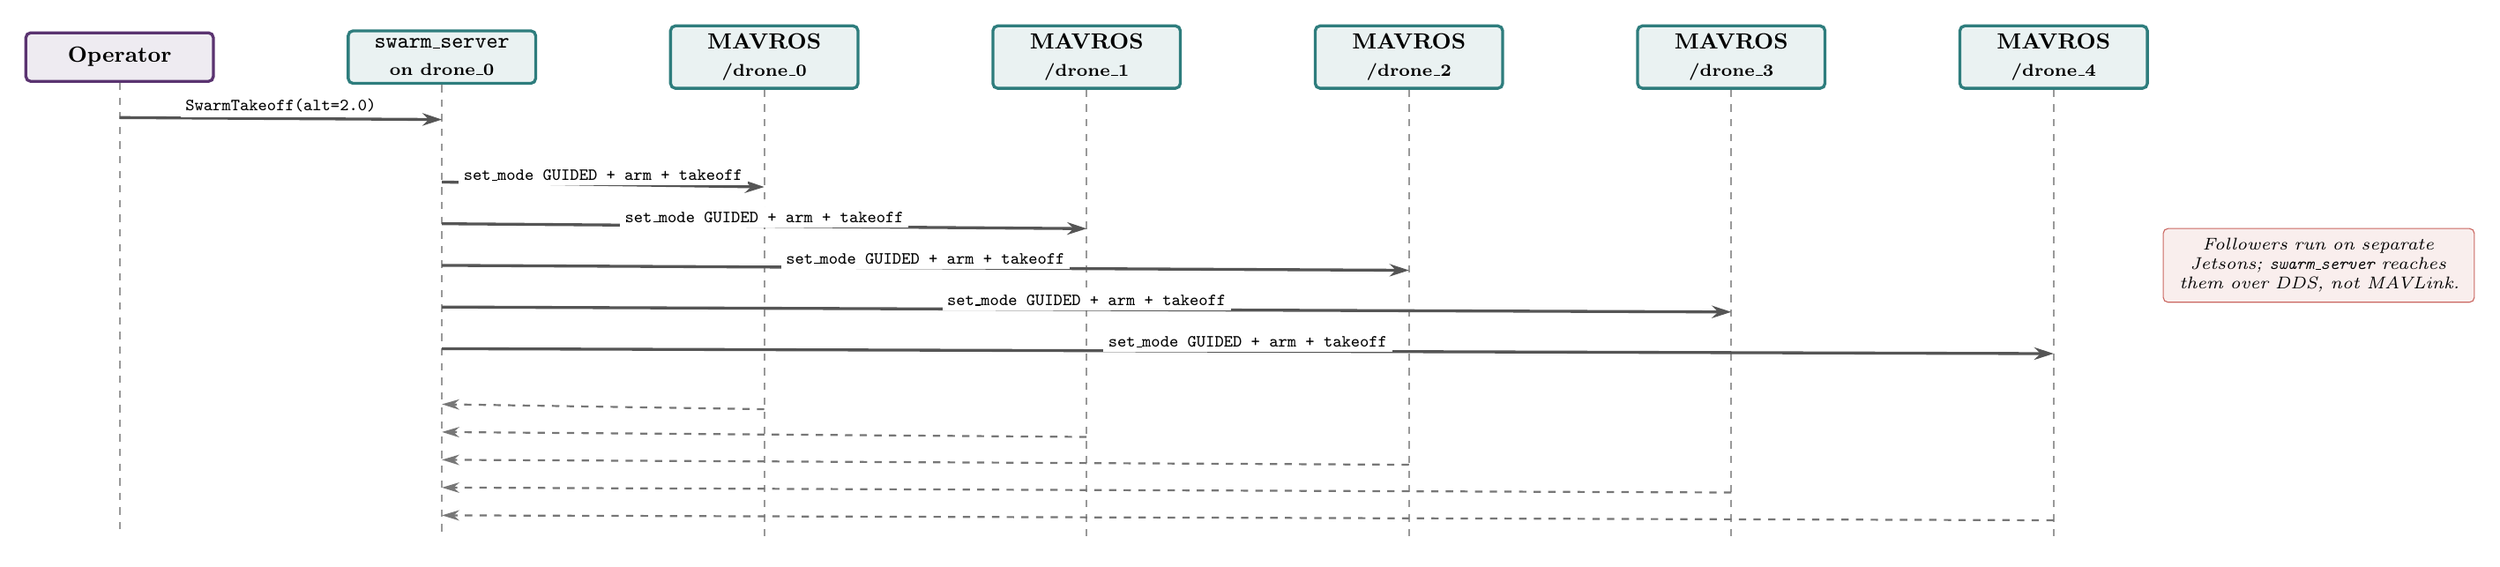
\begin{tikzpicture}[node distance=1.9cm]
  \node[sdactorops] (op) {Operator};
  \node[sdactorlight, right=of op] (ss) {\texttt{swarm\_server}\\\scriptsize on drone\_0};
  \node[sdactorlight, right=of ss] (m0) {MAVROS\\\scriptsize /drone\_0};
  \node[sdactorlight, right=of m0] (m1) {MAVROS\\\scriptsize /drone\_1};
  \node[sdactorlight, right=of m1] (m2) {MAVROS\\\scriptsize /drone\_2};
  \node[sdactorlight, right=of m2] (m3) {MAVROS\\\scriptsize /drone\_3};
  \node[sdactorlight, right=of m3] (m4) {MAVROS\\\scriptsize /drone\_4};

  \foreach \n in {op, ss, m0, m1, m2, m3, m4} {
    \draw[lifeline] (\n.south) -- ++(0,-6.5);
  }

  \draw[sdmsg] ($(op.south) + (0,-0.5)$) -- node[sdlab, above]{SwarmTakeoff(alt=2.0)} ($(ss.south) + (0,-0.5)$);

  \foreach \i/\m in {1.4/m0, 2.0/m1, 2.6/m2, 3.2/m3, 3.8/m4} {
    \draw[sdmsg] ($(ss.south) + (0,-\i)$) -- node[sdlab, above, yshift=-1pt]{set\_mode GUIDED + arm + takeoff} ($(\m.south) + (0,-\i)$);
  }

  \foreach \i/\m in {4.6/m0, 5.0/m1, 5.4/m2, 5.8/m3, 6.2/m4} {
    \draw[sdret] ($(\m.south) + (0,-\i)$) -- ($(ss.south) + (0,-\i)$);
  }

  \node[notebox, anchor=west, text width=4.2cm] at ($(m4.east) + (0.2,-3.0)$)
    {Followers run on separate Jetsons; \texttt{swarm\_server} reaches them over DDS, not MAVLink.};
\end{tikzpicture}%
}
\end{center}

\subsection{The leader-pose watchdog --- state machine}

\begin{center}
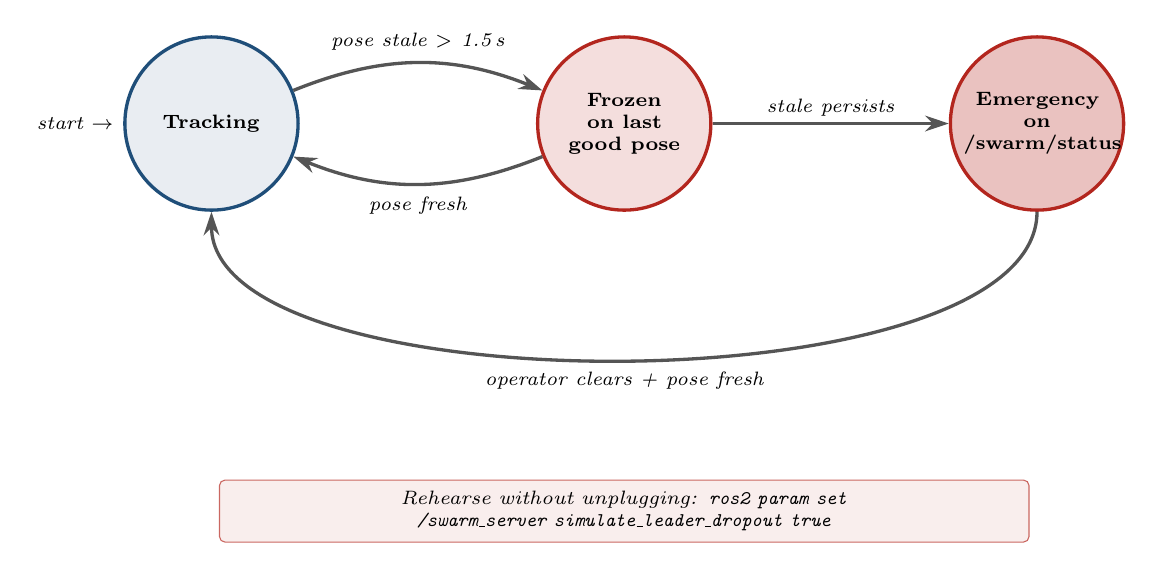
\begin{tikzpicture}[node distance=3.0cm,
    swstate/.style={circle, draw=fcblue, very thick, fill=fcblue!10,
                    font=\scriptsize\bfseries, align=center, text width=1.8cm, inner sep=1pt,
                    minimum size=2.2cm},
    swstatealert/.style={circle, draw=warnred, very thick, fill=warnred!15,
                         font=\scriptsize\bfseries, align=center, text width=1.8cm, inner sep=1pt,
                         minimum size=2.2cm},
    swstateemerg/.style={circle, draw=warnred, very thick, fill=warnred!28,
                         font=\scriptsize\bfseries, align=center, text width=1.8cm, inner sep=1pt,
                         minimum size=2.2cm}]
  \node[swstate] (track) {Tracking};
  \node[swstatealert, right=of track] (frozen) {Frozen on last good pose};
  \node[swstateemerg, right=of frozen] (emerg) {Emergency on /swarm/status};

  \draw[link, bend left=22] (track) to node[linklabel, above, yshift=2pt]{pose stale $>$ 1.5\,s} (frozen);
  \draw[link, bend left=22] (frozen) to node[linklabel, below, yshift=-2pt]{pose fresh} (track);
  \draw[link] (frozen) to node[linklabel, above]{stale persists} (emerg);
  % return arc loops well below all three states
  \draw[link] (emerg.south) .. controls ($(emerg.south) + (0,-2.5)$)
                              and ($(track.south) + (0,-2.5)$)
                              .. node[linklabel, below=2pt, pos=0.5]{operator clears + pose fresh}
                              (track.south);

  \node[anchor=east, font=\scriptsize\itshape] at (track.west) {start $\rightarrow$};

  \node[notebox, below=3.4cm of frozen, text width=10cm]
    {Rehearse without unplugging: \texttt{ros2 param set /swarm\_server simulate\_leader\_dropout true}};
\end{tikzpicture}
\end{center}

\begin{tcolorbox}[colback=accentgreen!8, colframe=accentgreen, boxrule=0.8pt, arc=2pt]
\textbf{Gate to leave Stage E:} \texttt{/swarm/takeoff} switches \emph{every} FC
to GUIDED (or refuses to arm if no GPS --- same on every drone). The simulated
watchdog dropout raises the emergency on \texttt{/swarm/status} within 1.5 s.
\end{tcolorbox}

\newpage

% =================================================================
% STAGE F
% =================================================================
\section{Stage F --- First hover, then two-drone leader-follow}
\stagebanner{F}{Props on, one or two drones}{validate the airframe and the role separation before scaling to five.}

\subsection{Authority hierarchy --- who can override whom}

\begin{center}
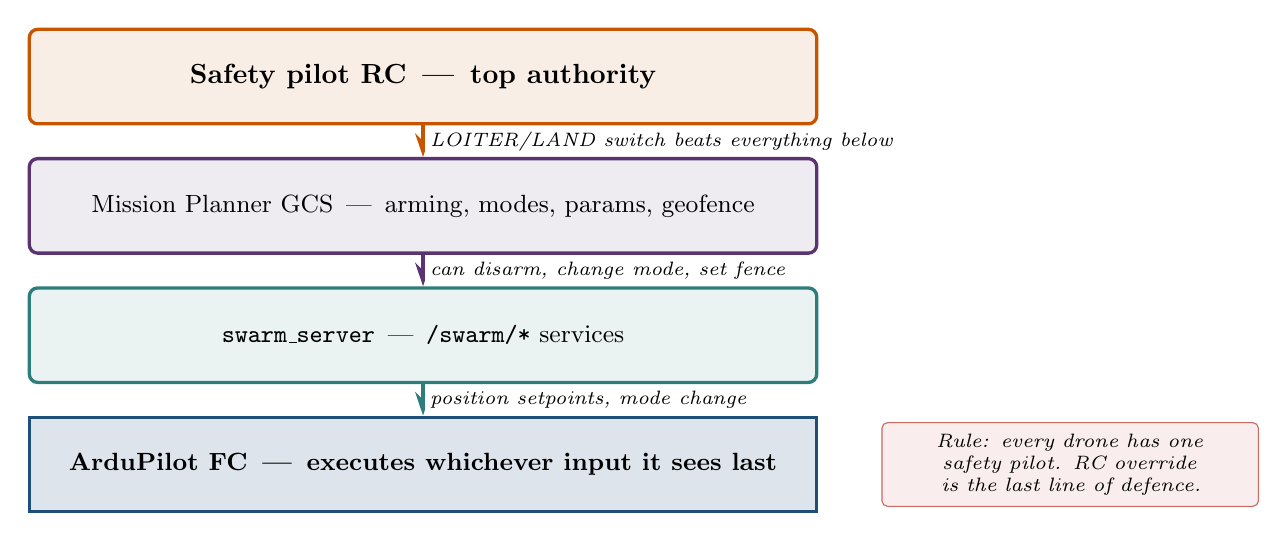
\begin{tikzpicture}[node distance=0.4cm]
  \node[rcbox, minimum width=10cm, minimum height=1.2cm, font=\bfseries]
    (rc) {Safety pilot RC \,---\, top authority};
  \node[gcsbox, below=of rc, minimum width=10cm, minimum height=1.2cm]
    (mp) {Mission Planner GCS \,---\, arming, modes, params, geofence};
  \node[jetbox, below=of mp, minimum width=10cm, minimum height=1.2cm]
    (ss) {\texttt{swarm\_server} \,---\, \texttt{/swarm/*} services};
  \node[fcbox, below=of ss, minimum width=10cm, minimum height=1.2cm]
    (fc) {ArduPilot FC \,---\, executes whichever input it sees last};

  \draw[link, draw=rcorange] (rc.south) -- node[linklabel, right]{LOITER/LAND switch beats everything below} (mp.north);
  \draw[link, draw=gcspurple] (mp.south) -- node[linklabel, right]{can disarm, change mode, set fence} (ss.north);
  \draw[link, draw=jetsonteal] (ss.south) -- node[linklabel, right]{position setpoints, mode change} (fc.north);

  \node[notebox, right=0.8cm of fc, text width=4.5cm, anchor=west]
    {Rule: every drone has one safety pilot. RC override is the last line of defence.};
\end{tikzpicture}
\end{center}

\subsection{Leader-follow data flow (two drones)}

\begin{center}
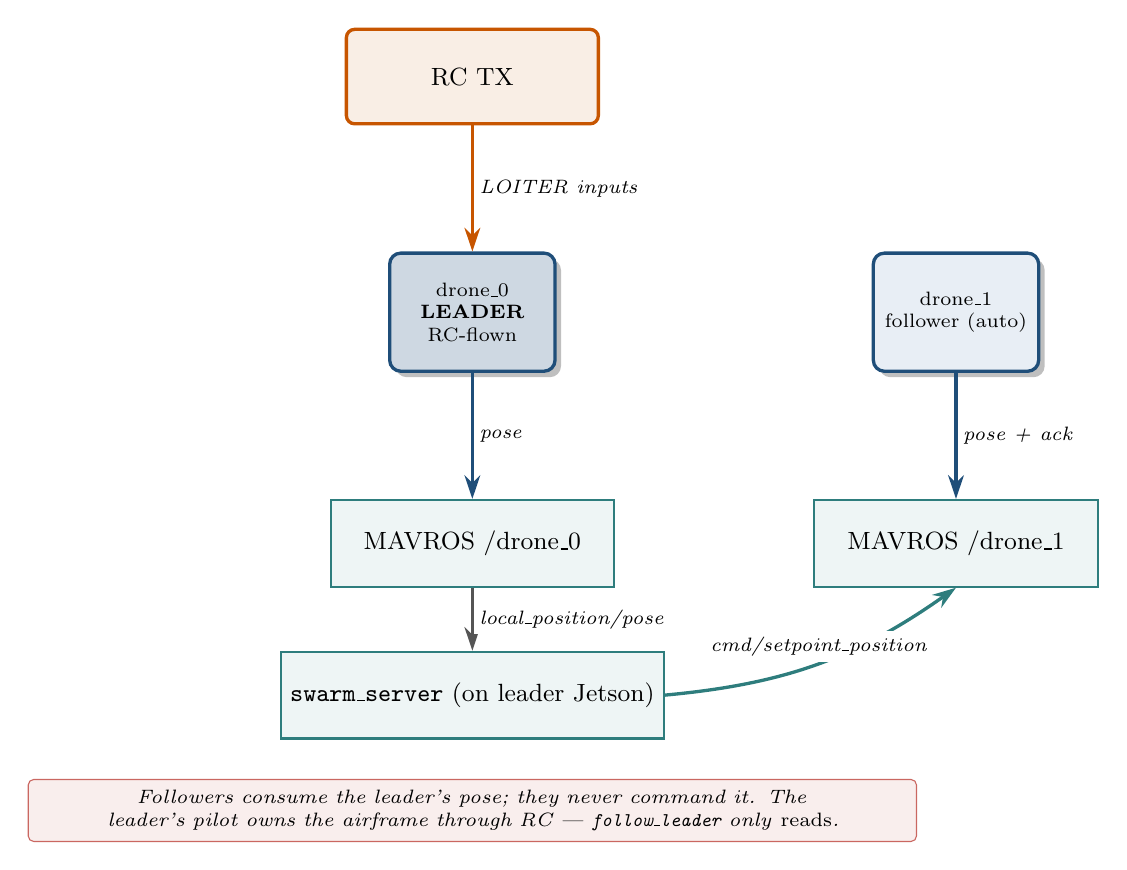
\begin{tikzpicture}[node distance=1.6cm]
  \node[drone, fill=fcblue!22] (d0) {drone\_0\\\textbf{LEADER}\\\scriptsize RC-flown};
  \node[drone, right=4cm of d0] (d1) {drone\_1\\\scriptsize follower (auto)};

  \node[swcomp, below=of d0] (m0) {MAVROS /drone\_0};
  \node[swcomp, below=of d1] (m1) {MAVROS /drone\_1};
  \node[swcomp, below=0.8cm of m0] (ss) {\texttt{swarm\_server} (on leader Jetson)};

  \draw[link, draw=fcblue] (d0.south) -- node[linklabel, right]{pose} (m0.north);
  \draw[link, draw=fcblue] (d1.south) -- node[linklabel, right]{pose + ack} (m1.north);
  \draw[link] (m0.south) -- node[linklabel, right]{local\_position/pose} (ss.north);
  \draw[link, draw=jetsonteal, bend right=15] (ss.east) to node[linklabel, above]{cmd/setpoint\_position} (m1.south);

  \node[rcbox, above=of d0] (rc) {RC TX};
  \draw[link, draw=rcorange] (rc.south) -- node[linklabel, right]{LOITER inputs} (d0.north);

  \node[notebox, below=0.5cm of ss, text width=11cm]
    {Followers consume the leader's pose; they never command it. The leader's
    pilot owns the airframe through RC --- \texttt{follow\_leader} only \emph{reads}.};
\end{tikzpicture}
\end{center}

\subsection{Two-drone leader-follow procedure}

\begin{enumerate}[leftmargin=*, itemsep=2pt]
  \item Props on drone\_0 and drone\_1 only. Drones 2--4 stay grounded with props off but powered (keep proving DDS health).
  \item \texttt{make demo-check} --- gate must say PREFLIGHT PASS.
  \item \texttt{/swarm/takeoff alt=4.0} --- both drones lift to 4 m hover in GUIDED.
  \item Drone\_0's safety pilot flips RC to \textbf{LOITER}. Drone\_0 is now hand-flown.
  \item \texttt{/swarm/follow\_leader enable=true formation=line spacing=5.0} --- drone\_1 tracks drone\_0's live pose.
  \item Leader pilot flies a slow box; watch \texttt{/swarm/formation\_error} on Foxglove.
  \item \texttt{/swarm/follow\_leader enable=false}; leader lands on RC; \texttt{/swarm/land} for drone\_1.
\end{enumerate}

\begin{tcolorbox}[colback=accentgreen!8, colframe=accentgreen, boxrule=0.8pt, arc=2pt]
\textbf{Gate to leave Stage F:} two drones complete the leader-follow box with
\texttt{formation\_error} remaining below your acceptable threshold (start at 2 m).
\end{tcolorbox}

\newpage

% =================================================================
% STAGE G
% =================================================================
\section{Stage G --- Full five-drone diamond}
\stagebanner{G}{Five drones in the air, in formation}{the end-state of Phase 2.5b.}

\subsection{Field setup --- top-down}

\begin{center}
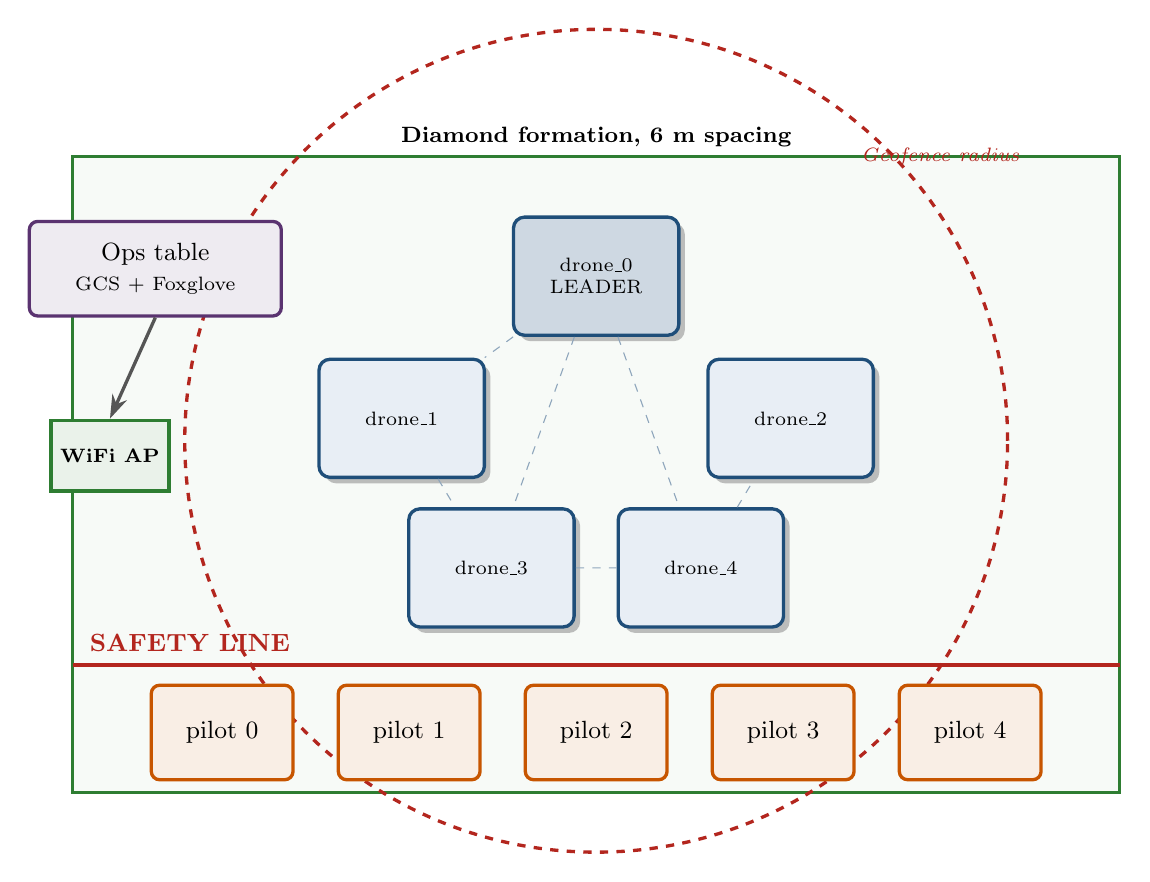
\begin{tikzpicture}[scale=0.95]
  % field outline
  \draw[draw=accentgreen, very thick, fill=accentgreen!4]
    (-7,-5.5) rectangle (7,3);

  % geofence circle
  \draw[draw=warnred, dashed, very thick] (0,-0.8) circle (5.5);
  \node[font=\scriptsize\itshape, anchor=south west] at (3.4,3.4) {};
  \node[font=\scriptsize\itshape\color{warnred}] at (4.6,3.0) {Geofence radius};

  % diamond positions
  \node[drone, fill=fcblue!22] (Ld) at (0,1.4) {drone\_0\\LEADER};
  \node[drone] (Lt) at (-2.6,-0.5) {drone\_1};
  \node[drone] (Rt) at (2.6,-0.5) {drone\_2};
  \node[drone] (Lb) at (-1.4,-2.5) {drone\_3};
  \node[drone] (Rb) at (1.4,-2.5) {drone\_4};

  \draw[dashed, draw=fcblue!50] (Ld) -- (Lt) -- (Lb) -- (Rb) -- (Rt) -- cycle;
  \draw[dashed, draw=fcblue!50] (Ld) -- (Lb);
  \draw[dashed, draw=fcblue!50] (Ld) -- (Rb);

  % safety line
  \draw[ultra thick, draw=warnred] (-7,-3.8) -- (7,-3.8);
  \node[anchor=south west, font=\small\bfseries\color{warnred}] at (-6.9,-3.75) {SAFETY LINE};

  % roles on the safety side
  \node[rcbox, minimum width=1.8cm] (rc0) at (-5,-4.7) {pilot 0};
  \node[rcbox, minimum width=1.8cm] (rc1) at (-2.5,-4.7) {pilot 1};
  \node[rcbox, minimum width=1.8cm] (rc2) at (0,-4.7) {pilot 2};
  \node[rcbox, minimum width=1.8cm] (rc3) at (2.5,-4.7) {pilot 3};
  \node[rcbox, minimum width=1.8cm] (rc4) at (5,-4.7) {pilot 4};

  \node[gcsbox, anchor=west, minimum width=3.2cm, minimum height=1.2cm] (ops) at (-7.6,1.5) {Ops table\\\scriptsize GCS + Foxglove};
  \node[draw=accentgreen, very thick, fill=accentgreen!10, minimum width=1.4cm,
        minimum height=0.9cm, font=\scriptsize\bfseries, align=center] (ap)
    at (-6.5,-1) {WiFi AP};

  \draw[link] (ops.south) -- (ap.north);

  \node[font=\footnotesize\bfseries, anchor=south] at (0,3.0) {Diamond formation, 6 m spacing};
\end{tikzpicture}
\end{center}

\subsection{Role assignment}

\begin{center}
\renewcommand{\arraystretch}{1.25}
\begin{tabularx}{15cm}{lX}
\toprule
\textbf{Role} & \textbf{Responsibility} \\
\midrule
\textbf{Leader pilot} & RC-fly drone\_0 in LOITER through a slow, pre-briefed pattern. Calls abort if any follower drifts unsafely. \\
\textbf{Follower pilots} (\,$\times 4$\,) & One per drone. Hand on the transmitter. RC override to LOITER or LAND on cue or on any unsafe behaviour. \\
\textbf{Swarm operator} & Issues \texttt{/swarm/*} service calls from the ops laptop. Watches \texttt{/swarm/status} and \texttt{/swarm/formation\_error}. \\
\textbf{Safety officer} & Outside the loop; calls "abort" verbally when the pre-briefed envelope is breached. \\
\bottomrule
\end{tabularx}
\end{center}

\subsection{The flight, condensed}

\begin{enumerate}[leftmargin=*, itemsep=2pt]
  \item Preflight gate on the leader Jetson: \texttt{make demo-check} $\rightarrow$ PREFLIGHT PASS.
  \item Five pilots in position, transmitters live, callouts ready.
  \item \texttt{/swarm/takeoff alt=5.0}.
  \item Leader pilot flips to LOITER.
  \item \texttt{/swarm/follow\_leader enable=true formation=diamond spacing=6.0}.
  \item Leader pilot flies the pre-briefed pattern; ops watches formation error.
  \item \texttt{/swarm/follow\_leader enable=false}.
  \item Leader lands on RC; \texttt{/swarm/land} for followers.
\end{enumerate}

\photoplaceholder{14}{5}{Five-drone diamond formation in the air, safety line and pilots visible in the foreground. Captured during the Phase 2.5b flight.}

\begin{tcolorbox}[colback=accentgreen!8, colframe=accentgreen, boxrule=0.8pt, arc=2pt]
\textbf{Gate to leave Stage G:} all five drones complete the briefed pattern,
land cleanly, no RTL triggered, no RC override used in anger. Phase 2.5b
complete.
\end{tcolorbox}

\newpage

% =================================================================
% FAILURE MODES
% =================================================================
\section{Failure modes mapped to gates}

Each failure has exactly one stage that should catch it. If a problem first
appears \emph{after} its catching stage, you skipped the gate.

\begin{center}
\renewcommand{\arraystretch}{1.3}
\begin{tabularx}{16cm}{p{2.5cm}p{5cm}X}
\toprule
\textbf{First caught at} & \textbf{Failure mode} & \textbf{Where it manifests} \\
\midrule
\textbf{Stage A} & TX/RX swapped, baud mismatch, getty holding port, FC unpowered & \texttt{fc\_link\_test.py} prints no heartbeat; \texttt{make demo-up} healthcheck times out \\
\textbf{Stage A} & Wrong L4T release (R32 instead of R36) & Base-image build fails or container exits immediately \\
\textbf{Stage A} & ArduPilot params not written / not rebooted & FC connects but rejects \texttt{set\_mode GUIDED}; geofence default-off \\
\textbf{Stage B} & Overlay build broken (\texttt{swarm\_msgs} IDL drift, missing dep) & Container exits before MAVROS launch; check \texttt{/tmp/overlay\_log} \\
\textbf{Stage C} & AP drops multicast / has client isolation & \texttt{\_\_dds\_probe} silent from peer; topic list shows only local node \\
\textbf{Stage C} & Wrong \texttt{NetworkInterfaceAddress} & DDS picks loopback or eth, never WiFi --- no peers seen \\
\textbf{Stage C} & Duplicate IP on the LAN & DDS sees half the swarm; \texttt{ros2 node list} is unstable \\
\textbf{Stage D} & Duplicate \texttt{SYSID\_THISMAV} & One MAVROS silently drops; \texttt{demo-check} names the missing drone \\
\textbf{Stage D} & Compass / EKF not calibrated & EKF origin never sets; preflight blocks on that drone \\
\textbf{Stage D} & \texttt{SRn\_*} stream rates wrong for the wired port & \texttt{local\_position/pose} silent on that drone; follower cannot track \\
\textbf{Stage E} & Watchdog timing not what you expected & Simulated dropout does not raise emergency in 1.5 s; tune \texttt{LEADER\_POSE\_TIMEOUT} \\
\textbf{Stage F} & PID tune wrong for airframe & Drone oscillates in hover; abort, retune in Mission Planner \\
\textbf{Stage F} & Geofence radius too tight for formation spacing & Followers RTL on engage; widen \texttt{FENCE\_RADIUS} \\
\textbf{Stage G} & Operator coordination breakdown & Safety officer abort; debrief, rehearse the choreography \\
\bottomrule
\end{tabularx}
\end{center}

\newpage

% =================================================================
% DAY ONE
% =================================================================
\section{What to do, tomorrow}

\begin{center}
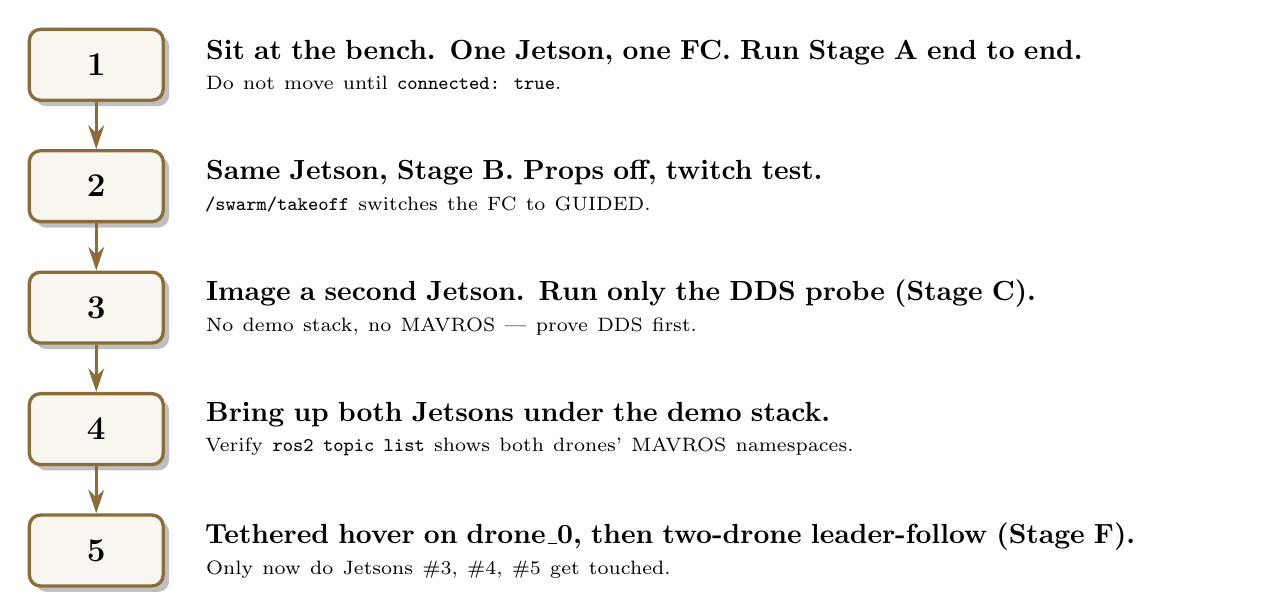
\begin{tikzpicture}[node distance=0.6cm]
  \node[stagebadge] (1) {1};
  \node[right=0.4cm of 1, anchor=west, align=left, text width=13cm]
    {\textbf{Sit at the bench. One Jetson, one FC. Run Stage A end to end.} \\[-1pt]
     \scriptsize Do not move until \texttt{connected: true}.};
  \node[stagebadge, below=of 1] (2) {2};
  \node[right=0.4cm of 2, anchor=west, align=left, text width=13cm]
    {\textbf{Same Jetson, Stage B. Props off, twitch test.} \\[-1pt]
     \scriptsize \texttt{/swarm/takeoff} switches the FC to GUIDED.};
  \node[stagebadge, below=of 2] (3) {3};
  \node[right=0.4cm of 3, anchor=west, align=left, text width=13cm]
    {\textbf{Image a second Jetson. Run only the DDS probe (Stage C).} \\[-1pt]
     \scriptsize No demo stack, no MAVROS --- prove DDS first.};
  \node[stagebadge, below=of 3] (4) {4};
  \node[right=0.4cm of 4, anchor=west, align=left, text width=13cm]
    {\textbf{Bring up both Jetsons under the demo stack.} \\[-1pt]
     \scriptsize Verify \texttt{ros2 topic list} shows both drones' MAVROS namespaces.};
  \node[stagebadge, below=of 4] (5) {5};
  \node[right=0.4cm of 5, anchor=west, align=left, text width=13cm]
    {\textbf{Tethered hover on drone\_0, then two-drone leader-follow (Stage F).} \\[-1pt]
     \scriptsize Only now do Jetsons \#3, \#4, \#5 get touched.};

  \draw[->, very thick, >={Stealth[length=3mm,width=2mm]}, draw=stagerule]
    (1) -- (2);
  \draw[->, very thick, >={Stealth[length=3mm,width=2mm]}, draw=stagerule]
    (2) -- (3);
  \draw[->, very thick, >={Stealth[length=3mm,width=2mm]}, draw=stagerule]
    (3) -- (4);
  \draw[->, very thick, >={Stealth[length=3mm,width=2mm]}, draw=stagerule]
    (4) -- (5);
\end{tikzpicture}
\end{center}

\vspace{0.6cm}

\noindent\textbf{The point.} The catalogue of failure modes in §8 is long.
The bring-up sequence is what makes that list \emph{shrink}: each stage takes
one item off the list before the next stage's failures can hide behind it.
Five drones in the air on the first try is a fluke; five drones in the air on
the first try \emph{after} stages A--F is the engineering.

\vspace{1.2cm}

\hrulefill

\vspace{0.4cm}

\noindent\small\textit{References.}
\begin{itemize}[leftmargin=*, itemsep=1pt]
  \item \texttt{docs/architecture/end\_to\_end/end\_to\_end\_setup.pdf} --- architecture, UML, network topology, field setup.
  \item \texttt{docs/runbooks/jetson\_swarm\_operations.md} --- per-step command reference and troubleshooting matrix.
  \item \texttt{docs/runbooks/first\_flight.md} --- the Phase 2.5b flight procedure (safety gate, roles, aborts).
  \item \texttt{config/networks/cyclonedds\_drone\_template.xml} --- the DDS peer-list template (§5).
  \item \texttt{config/ardupilot\_params/README.md} --- the param-load procedure used in Stage A.
  \item \texttt{scripts/hardware/fc\_link\_test.py} --- pure pymavlink bench probe (Stage A).
\end{itemize}

\end{document}
